\section{Details of the Reviewing Process}
\label{app:review-details}

In this section, for reference, we provide some details on the reviewing process for NeurIPS 2014. We include time line, and the paper scoring instructions. Reviewer instructions and paper scoring evolve over the years for NeurIPS. Broadly speaking, the instructions for the 2014 edition of the conference remained the same as the 2013 edition, with additional stipulations given for those who's papers were selected for the NeurIPS experiment.

The timeline for the conference is given in Table \ref{table-reviewing-timeline}.


\begin{table}[hb]
    \centering
    \caption{Timeline for the 2014 conference. Dates are each given in ISO format. Timeline broadly matched that used in previous years of the conference.}
    \label{table-reviewing-timeline}
    
    \begin{tabular}{l|r}
    Event & Date \\ \hline
    
        Submission Deadline & 2014-06-06  \\
        Bidding Open for Area Chairs (this was \emph{delayed} by
  CMT issues) & 2014-06-12 \\
  Bidding Open for Reviewers & 2014-06-17 \\
  Start Reviewing & 2014-07-01 \\
  Reviewing deadline & 2014-07-21 \\
  Reviews to Authors & 2014-08-04 \\
  Author Rebuttal Due & 2014-08-11 \\
  Teleconferences Begin & 2014-08-25 \\
  Teleconferences End & 2014-08-30 \\
  Preliminary Decisions Made & 2014-09-01 \\
  Decisions Sent to Authors & 2014-09-09
    \end{tabular}
    
\end{table}

\subsection{Paper Scoring and Reviewer
Instructions}\label{paper-scoring-and-reviewer-instructions}

To keep quality of reviews high, we tried to keep reviewing load low. We didn't
assign any reviewer more than 5 papers, most reviewers received 4
papers.
The instructions to reviewers for the 2014 conference are 
available online\footnote{See  
\url{https://neurips.cc/Conferences/2014/PaperInformation/ReviewerInstructions}} and we summarise also below.

The reviewers assign a number of scores: Quantitative Evaluation,
Impact Score, Confidence Score, and a verbal Qualitative Evaluation to
each paper they review. For detail about these 4 assessments, see below.

\subsection*{Quantitative Evaluation}
Reviewers give a score of between 1 and 10 for each paper. The program
committee will interpret the numerical score in the following way:

\begin{description}
\item[10] Top 5\% of accepted NeurIPS papers, a seminal paper for the ages.

  I will consider not reviewing for NeurIPS again if this is rejected.
\item[9] Top 15\% of accepted NeurIPS papers, an excellent paper, a strong
  accept.

  I will fight for acceptance.
\item[8] Top 50\% of accepted NeurIPS papers, a very good paper, a clear
  accept.

  I vote and argue for acceptance.
\item[7] Good paper, accept.

  I vote for acceptance, although would not be upset if it were
  rejected.
\item[6] Marginally above the acceptance threshold.

  I tend to vote for accepting it, but leaving it out of the program
  would be no great loss.
\item[5] Marginally below the acceptance threshold.

  I tend to vote for rejecting it, but having it in the program would
  not be that bad.
\item[4] An OK paper, but not good enough. A rejection.

  I vote for rejecting it, although would not be upset if it were
  accepted.
\item[3] A clear rejection.

  I vote and argue for rejection.
\item[2] A strong rejection. I'm surprised it was submitted to this
  conference.

  I will fight for rejection.
\item[1] Trivial or wrong or known. I'm surprised anybody wrote such a
  paper.

  I will consider not reviewing for NeurIPS again if this is accepted.
\end{description}

Reviewers should NOT assume that they have received an unbiased sample
of papers, nor should they adjust their scores to achieve an artificial
balance of high and low scores. Scores should reflect absolute judgments
of the contributions made by each paper.

\subsection*{Impact Score}\label{impact-score}

The impact score was an innovation introduce in 2013 by Ghahramani and
Welling that we retained for 2014. 

Independently of the Quality Score above, this is your opportunity to
identify papers that are very different, original, or otherwise
potentially impactful for the NeurIPS community.

There are two choices:

\begin{description}
\item[2] This work is different enough from typical submissions to potentially
have a major impact on a subset of the NeurIPS community.

\item[1] This work is incremental and unlikely to have much impact even though
it may be technically correct and well executed.
\end{description}

Examples of situations where the impact and quality scores may point in
opposite directions include papers which are technically strong but
unlikely to generate much follow-up research, or papers that have some
flaw (e.g.~not enough evaluation, not citing the right literature) but
could lead to new directions of research.


\subsection*{Confidence Score}\label{confidence-score}

Reviewers also give a confidence score between 1 and 5 for each paper.
The program committee will interpret the numerical score in the
following way:

\begin{description}
\item[5] The reviewer is absolutely certain that the evaluation is correct and
very familiar with the relevant literature.

\item[4] The reviewer is confident but not absolutely certain that the
evaluation is correct. It is unlikely but conceivable that the reviewer
did not understand certain parts of the paper, or that the reviewer was
unfamiliar with a piece of relevant literature.

\item[3] The reviewer is fairly confident that the evaluation is correct. It
is possible that the reviewer did not understand certain parts of the
paper, or that the reviewer was unfamiliar with a piece of relevant
literature. Mathematics and other details were not carefully checked.

\item[2] The reviewer is willing to defend the evaluation, but it is quite
likely that the reviewer did not understand central parts of the paper.

\item[1] The reviewer's evaluation is an educated guess. Either the paper is
not in the reviewer's area, or it was extremely difficult to understand.
\end{description}

\subsection*{Qualitative Evaluation}\label{qualitative-evaluation}

All NeurIPS papers should be good scientific papers, regardless of their
specific area. We judge whether a paper is good using four criteria; a
reviewer should comment on all of these, if possible:

\begin{itemize}
\item
  Quality

  Is the paper technically sound? Are claims well-supported by
  theoretical analysis or experimental results? Is this a complete piece
  of work, or merely a position paper? Are the authors careful (and
  honest) about evaluating both the strengths and weaknesses of the
  work?
\item
  Clarity

  Is the paper clearly written? Is it well-organized? (If not, feel free
  to make suggestions to improve the manuscript.) Does it adequately
  inform the reader? (A superbly written paper provides enough
  information for the expert reader to reproduce its results.)
\item
  Originality

  Are the problems or approaches new? Is this a novel combination of
  familiar techniques? Is it clear how this work differs from previous
  contributions? Is related work adequately referenced? We recommend
  that you check the proceedings of recent NeurIPS conferences to make sure
  that each paper is significantly different from papers in previous
  proceedings. Abstracts and links to many of the previous NeurIPS papers
  are available from http://books.NeurIPS.cc
\item
  Significance
  
  Are the results important? Are other people (practitioners or
  researchers) likely to use these ideas or build on them? Does the paper
  address a difficult problem in a better way than previous research? Does
  it advance the state of the art in a demonstrable way? Does it provide
  unique data, unique conclusions on existing data, or a unique
  theoretical or pragmatic approach?
\end{itemize}

\section{Code and Data}

All code for our experiments can be found on line in Jupyter notebooks, \url{https://github.com/lawrennd/neurips2014/} and an accompanying python package for dealing with the data \url{https://github.com/lawrennd/cmtutils/}, it can be installed with `pip install cmtutils`. Code was all originally written in Python 2, but is now updated for compatibility with Python 3.

The repository has all the code used for managing the NeurIPS reviewing process in a set of different notebooks. The relevant notebooks for recreating the different experiments below are listed in each section.

Unfortunately, the full data for recreating our analysis is not public, due to challenges around anonymizing reviewer identity and the identity of authors whose papers weren't accepted at the conference.

\section{NeurIPS Experiment Results}
\label{app:neurips-experiment-results}

The results of the experiment are listed in Table~\ref{table-neurips-experiment-results} in the main body of the paper. A Jupyter notebook for recreating this analysis can be found here \url{https://github.com/lawrennd/neurips2014/blob/master/notebooks/The%20NIPS%20Experiment.ipynb}.

There are a few ways of summarising the numbers in this table as percent
or probabilities. First, the inconsistency is the proportion of decisions
that were not the same across the two committees. The decisions were
inconsistent for 43 out of 166 papers or 0.259 as a proportion. This
number is a natural way of summarising the figures if you are
submitting your paper and wish to know an estimate of what the
probability is that your paper would have different decisions according
to the different committees. 

Secondly, the accept precision: if you are
attending the conference and looking at any given paper, then you might
want to know the probability that the paper would have been rejected in
an independent rerunning of the conference. We can estimate this for
Committee 1's conference as 22/(22 + 22) = 0.5 (50\%) and for Committee
2's conference as 21/(22+21) = 0.49 (49\%). Averaging the two estimates
gives us 49.5\%. 

Thirdly, the reject precision: if your paper was
rejected from the conference, you might like an estimate of the
probability that the same paper would be rejected again if the review
process had been independently rerun. That estimate is 101/(22+101) =
0.82 (82\%) for Committee 1 and 101/(21+101)=0.83 (83\%) for Committee
2, or on average 82.5\%. 

A final quality estimate might be the ratio of
consistent accepts to consistent rejects, or the agreed accept rate,
22/123 = 0.18 (18\%).

\begin{itemize}
\tightlist
\item
  \emph{inconsistency}: 43/166 = \textbf{0.259}

  \begin{itemize}
  \tightlist
  \item
    proportion of decisions that were not the same
  \end{itemize}
\item
  \emph{accept precision} \(0.5 \times 22/44\) + \(0.5 \times 21/43\) =
  \textbf{0.495}

  \begin{itemize}
  \tightlist
  \item
    probability any accepted paper would be rejected in a rerunning
  \end{itemize}
\item
  \emph{reject precision} = \(0.5\times 101/(22+101)\) +
  \(0.5\times 101/(21 + 101)\) = \textbf{0.175}

  \begin{itemize}
  \tightlist
  \item
    probability any rejected paper would be rejected in a rerunning
  \end{itemize}
\item
  \emph{agreed accept rate} = 22/101 = \textbf{0.218}
  \begin{itemize}
    \item
  ratio between agreed accepted papers and agreed rejected papers.
  \end{itemize}
\end{itemize}

\subsection{Reaction After Experiment}\label{reaction-after-experiment}

There was a lot of discussion of the result, both at the
conference and on blogs and bulletin boards.\footnote{A summary of posts can be found here \url{https://inverseprobability.com/2015/01/16/blogs-on-the-nips-experiment}} Such discussion is to be
encouraged, and for ease of memory, it is worth pointing out that the
approximate proportions of papers in each category can be nicely divided
in to eighths as follows. Accept-Accept 1 in 8 papers, Accept-Reject 3
in 8 papers, Reject-Reject, 5 in 8 papers. This makes the statistics
we've computed above: inconsistency 1 in 4 (25\%) accept precision 1 in
2 (50\%) reject precision 5 in 6 (83\%) and agreed accept rate of 1 in 6
(20\%). This compares with the accept rate of 1 in 4.

\begin{itemize}
\item
  Public reaction after experiment is documented in a blog post.\footnote{\url{https://inverseprobability.com/2015/01/16/blogs-on-the-nips-experiment}}

\item
  NeurIPS was run in a very open way:
  code\footnote{\url{https://github.com/lawrennd/nips2014}} and
  blog
  posts\footnote{\url{https://inverseprobability.com/2014/12/16/the-nips-experiment}} all available.
\item
  Reaction triggered by a blog post from Eric Price.\footnote{\url{http://blog.mrtz.org/2014/12/15/the-nips-experiment.html}}
\end{itemize}

Much of the discussion following the conference speculated on the number of consistent accepts in
the process (using the main conference accept rate as a proxy). It
therefore produces numbers that don't match ours above. This is because
the computed accept rate of the individual committees is different from
that of the main conference. This could be due to a bias for the
duplicated papers, or statistical sampling error. To explore the issue, we do some statistics below. First, to get the reader primed for thinking about
these numbers we discuss some context for them.


\subsection{A Random Committee @ 25\% acceptance rate}\label{a-random-committee-25}
The first context we can place around the numbers is what would have
happened at the `random conference' where we simply accept a quarter of
papers at random. In this NeurIPS the expected numbers of accepts would
then have been given as in Table \ref{table-random-committee}.We consider a random committee that has a 25\% accept rate as it makes the numbers easier to remember and it's close to the observed accept rate of 23\%.

\begin{table}[htb]
\caption{Table shows the expected values for the confusion matrix if the committee was making decisions totally at random.}
\label{table-random-committee}
\centering


  \begin{tabular}{lc|c|c|}
  & & \multicolumn{2}{c}{Committee 1} \\
  & & Accept & Reject \\ \hline
  \multirow{2}{*}{Committee 2} & Accept & 10.4 (1 in 16) & 31.1 (3 in 16) \\ 
  & Reject & 31.1 (3 in 16) & 93.4 (9 in 16)
  \end{tabular}
\end{table}

And for this set up we would expect \emph{inconsistency} of 3 in 8
(37.5\%) \emph{accept precision} of 1 in 4 (25\%) and a \emph{reject
precision} of 3 in 4 (75\%) and a \emph{agreed accept rate} of 1 in 10
(10\%). The actual committee made improvements on these numbers, the
accept precision was markedly better with 50\%: twice as many consistent
accept decisions were made than would be expected if the process had
been performed at random and only around two thirds as many inconsistent
decisions were made as would have been expected if decisions were made
at random. However, we should treat all these figures with some
skepticism until we've performed some estimate of the uncertainty
associated with them (see Appendix~\ref{uncertainty-accept-rate}).



\section{Reviewer Calibration}
\label{app:reviewer-calibration}

Calibration of reviewers is the process where different interpretations
of the reviewing scale are addressed. Previous published models used for calibration include the model used in 2006 by John Platt \citep{Platt-calibration12} and the Bayesian variant used in 2013 by Welling and Ghahramani \cite{Ge-bayesian15}. You can find the code recreating our calibration in this Jupyter notebook \url{https://github.com/lawrennd/neurips2014/blob/master/notebooks/Reviewer%20Calibration.ipynb}.

At decision time for NeurIPS 2014, we didn't have access to the \cite{Ge-bayesian15} model and ended up proposing our own approach that turns out to also be a Bayesian interpretation of \cite{Platt-calibration12}. Our assumption is
that the score from the \(j\)th reviewer for the \(i\)th paper is given
by \[
y_{i,j} = f_i + b_j + \epsilon_{i, j},
\] 
where \(f_i\) is the `objective quality' of paper \(i\) and \(b_j\)
is an offset associated with reviewer \(j\). \(\epsilon_{i,j}\) is a
subjective quality estimate which reflects how a specific reviewer's
opinion differs from other reviewers (such differences in opinion may be
due to differing expertise or perspective). The underlying `objective
quality' of the paper is assumed to be the same for all reviewers and
the reviewer offset is assumed to be the same for all papers.

If we have \(n\) papers and \(m\) reviewers, then this implies \(n\) +
\(m\) + \(nm\) values need to be estimated. Naturally this is too many,
and we can start by assuming that the subjective quality is drawn from a
normal density with variance \(\sigma^2\) \[
\epsilon_{i, j} \sim N(0, \sigma^2 \mathbf{I})
\] which reduces us to \(n\) + \(m\) + 1 parameters. Further we can
assume that the objective quality is also normally distributed with mean
\(\mu\) and variance \(\alpha_f\), 
\[
f_i \sim N(\mu, \alpha_f)
\]
this now reduces us to \(m\)+3 parameters. However, we only have
approximately \(4m\) observations (4 papers per reviewer) so parameters
may still not be that well determined (particularly for those reviewers
that have only one paper to assess). We assume that reviewer
offset is normally distributed with zero mean, 
\[
b_j \sim N(0, \alpha_b),
\] 
leaving us only four parameters: \(\mu\), \(\sigma^2\), \(\alpha_f\)
and \(\alpha_b\). Combined together these three assumptions imply that
\[
\mathbf{y} \sim N(\mu \mathbf{1}, \mathbf{K}),
\]
where \(\mathbf{y}\) is a vector of stacked scores \(\mathbf{1}\) is
the vector of ones and the elements of the covariance function are given
by 
\[
k(i,j; k,l) = \delta_{i,k} \alpha_f + \delta_{j,l} \alpha_b + \delta_{i, k}\delta_{j,l} \sigma^2,
\] 
where $\delta_{\cdot,\cdot}$ is Kronecker delta function, \(i\) and \(j\) are the index of first paper and reviewer, and
\(k\) and \(l\) are the index of second paper and reviewer. The mean is
easily estimated by maximum likelihood and is given as the mean of all
scores.

We now reparametrize  to an overall scale
\(\alpha_f\), and normalized variance, \[
k(i,j; k,l) = \alpha_f\left(\delta_{i,k}  + \delta_{j,l} \frac{\alpha_b}{\alpha_f} + \delta_{i, k}\delta_{j,l} \frac{\sigma^2}{\alpha_f}\right)
\]
which we rewrite to give two ratios: offset/signal ratio,
\(\hat{\alpha}_b\) and noise/signal \(\hat{\sigma}^2\) ratio. \[
k(i,j; k,l) = \alpha_f\left(\delta_{i,k}  + \delta_{j,l} \hat{\alpha}_b + \delta_{i, k}\delta_{j,l} \hat{\sigma}^2\right).
\] 
The advantage of this parameterization is it allows us to optimize
\(\alpha_f\) with a fixed-point equation. This leaves us with two free parameters, that we can
explore on a grid. It is in these parameters that we expect the
remaining underdetermindness of the model. We expect \(\alpha_f\) to be
well determined because the negative log likelihood is now 
\[
\frac{|\mathbf{y}|}{2}\log\alpha_f + \frac{1}{2}\log  \left|\hat{\mathbf{K}}\right| + \frac{1}{2\alpha_f}\mathbf{y}^\top \hat{\mathbf{K}}^{-1} \mathbf{y},
\]
where \(|\mathbf{y}|\) is the length of \(\mathbf{y}\) (i.e.~the
number of reviews) and \(\hat{\mathbf{K}}=\alpha_f^{-1}\mathbf{K}\) is
the scale normalized covariance. This negative log likelihood is easily
minimized to recover 
\[
\alpha_f = \frac{1}{|\mathbf{y}|} \mathbf{y}^\top \hat{\mathbf{K}}^{-1} \mathbf{y}.
\] 
A Bayesian analysis of this parameter is possible with gamma priors,
but it would merely show that this parameter is extremely well
determined (the degrees of freedom parameter of the associated
Student-\(t\) marginal likelihood scales will the number of reviews,
which will be around \(|\mathbf{y}| \approx 6,000\) in our case).

So, we propose to proceed as follows. Set the mean from the reviews
(\(\mu\)) and then choose a two-dimensional grid of parameters for
reviewer offset and diversity. For each parameter choice, optimize to
find \(\alpha_f\) and then evaluate the likelihood. Worst case this will
require us inverting \(\hat{\mathbf{K}}\), but if the reviewer paper
groups are disconnected, it can be done a lot quicker.  In practice, we composed the model as a Gaussian process and use of the GPy software for parameter fitting \citep{Gpy-2012}. The full
analysis is described in a blog post.\footnote{\url{https://inverseprobability.com/2014/08/02/reviewer-calibration-for-nips}}.  The parameters of the fitted model are given in the main text in
Table \ref{table-fitted-calibration-parameters}.


\section{Uncertainty: Accept Rate}\label{uncertainty-accept-rate}

To get a handle on the uncertainty around these numbers we'll start by
making use of the
binomial distribution.
First, let's explore the fact that for the overall conference the accept
rate was around 23\%, but for the duplication committees the accept rate
was around 25\%. If we assume decisions are made according to a binomial
distribution, then is the accept rate for the duplicated papers too
high?

To reconstruct these examples or check for any errors in our code you can see our analysis in this Jupyter notebook: \url{https://github.com/lawrennd/neurips2014/blob/master/notebooks/The%20NIPS%20Experiment.ipynb}.

Note that for all our accept probability statistics we used as a
denominator the number of papers that were initially sent for review,
rather than the number where a final decision was made by the program
committee. These numbers are different because some papers are withdrawn
before the program committee makes its decision. Most commonly this
occurs after authors have seen their preliminary reviews: for NeurIPS 2014
we provided preliminary reviews that included paper scores. So for the
official accept probability we use the 170 as denominator. The accept
probabilities were therefore 43 out of 170 papers (25.3\%) for Committee
1 and 44 out of 170 (25.8\%) for Committee 2. This compares with the
overall conference accept rate for papers outside the duplication
process of 349 out of 1508 (23.1\%).

If the true underlying probability of an accept were 0.23, independent
of the paper, then the probability of generating accepts for any subset
of the papers would be given by a binomial distribution. Combining
across the two committees for the duplicated papers, we see that 87
papers in total were recommended for accept out of a total of 340
possible accepts. The shape of the binomial distribution for these values is 
depicted in Figure~\ref{fig:uncertainty-accept-rate} with the actual number of accepts being shown as a red line.


\begin{figure}[htb]
\centering
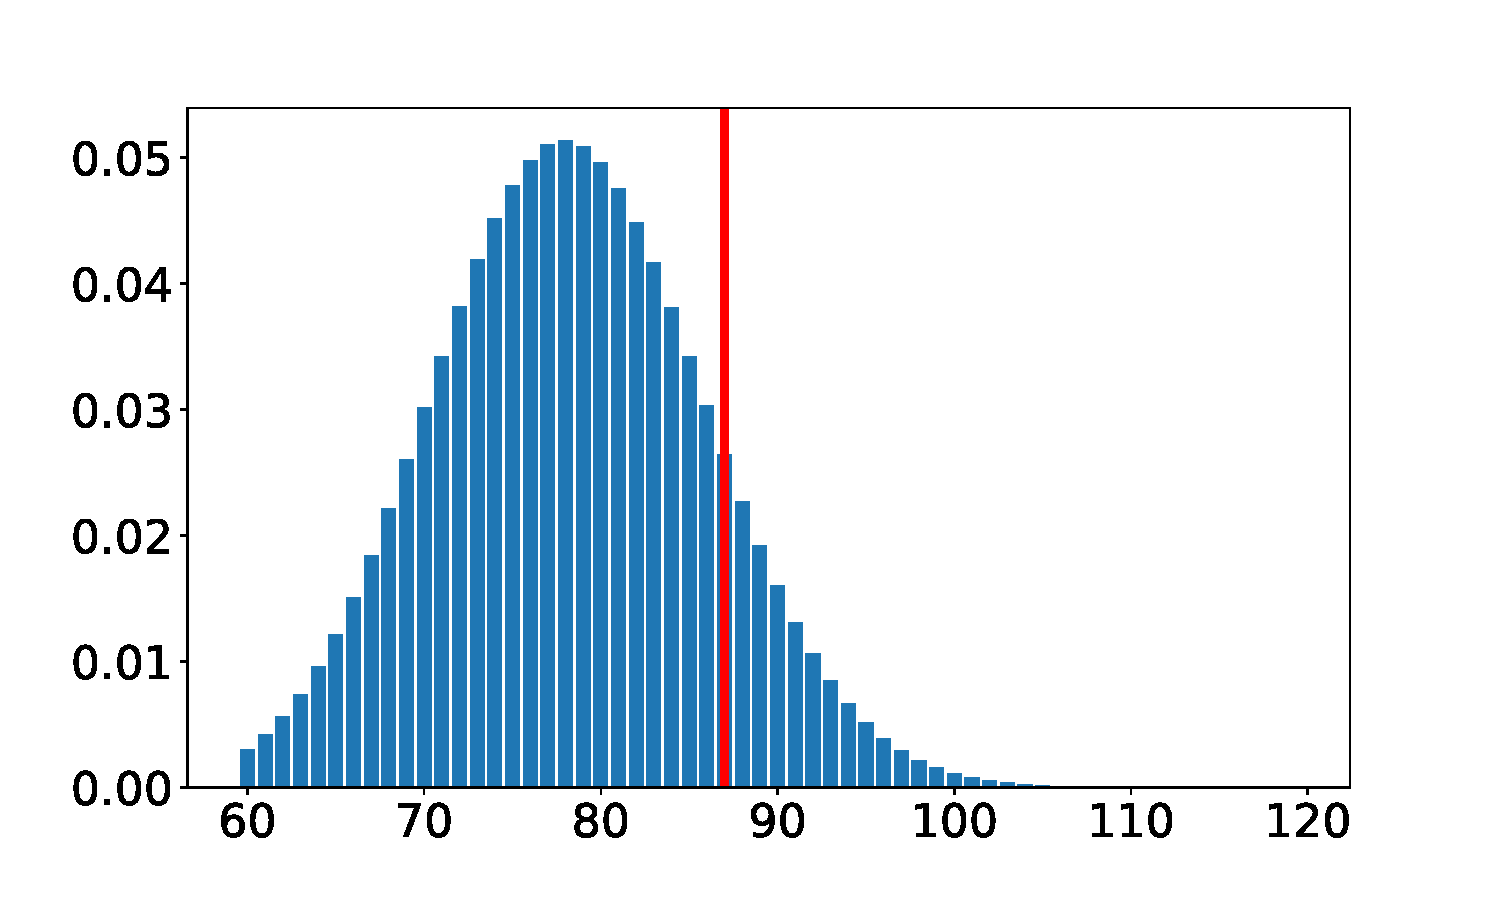
\includegraphics[width=0.70\textwidth]{diagrams/neurips/uncertainty-accept-rate.pdf}


\caption{Binomial distribution of the number of actual accepted papers we would observe if the true underlying accept probability was $p=0.23$ for all 340 decisions made by the two independent committees involved in the experiment. The observed number of accepted papers is given by a red line that falls well within the probability mass of the binomial.}
\label{fig:uncertainty-accept-rate}
\end{figure}

From the plot, we can see that whilst the accept rate was slightly
higher for duplicated papers it still falls well within the 
probability mass of the binomial distribution implied by a 0.23 accept rate.

Note that Area Chairs knew which papers were duplicates, whereas
reviewers did not. While we stipulated that duplicate papers should not
be any given special treatment, we cannot discount the possibility that
Area Chairs may have given slightly preferential treatment to duplicate
papers.

\subsection{Bayesian Analysis}\label{bayesian-analysis}

Before we start the analysis, it's important to make some statements
about the aims of our modelling here. We will make some simplifying
modelling assumptions for the sake of a model that is understandable. We
are looking to get a handle on the uncertainty associated with some of
the results of the NeurIPS experiment.
Some
preliminary analyses were conducted on blogs.\footnote{See \url{https://inverseprobability.com/2015/01/16/blogs-on-the-nips-experiment} for a summary.} Those
analyses don't have access to information like paper scores etc.. For
that reason we also leave out such information in this preliminary
analysis. We will focus only on the summary results from the experiment:
how many papers were consistently accepted, consistently rejected, or
had inconsistent decisions. For the moment we disregard the information
we have about paper scores.

In our analysis there are three possible outcomes for each paper:
consistent accept, inconsistent decision and consistent reject. So, we
need to perform the analysis with the
multinomial
distribution. The multinomial is parameterized by the probabilities of
the different outcomes. These are our parameters of interest; we would
like to estimate these probabilities alongside their uncertainties. For 
a Bayesian analysis we place a prior density over these
probabilities, then we update the prior with the observed data, that
gives us a posterior density, giving us an uncertainty associated with
these probabilities.

\subsection{Prior Density}\label{prior-density}

Choice of prior for the multinomial is typically straightforward, the Dirichlet
density is
conjugate and has
the additional advantage that its parameters can be set to ensure it is
\emph{uninformative}, i.e.~uniform across the domain of the prior.
Combination of a multinomial likelihood and a Dirichlet prior is not
new, and in this domain if we were to consider the mean the posterior
density only, then the approach is known as
Laplace
smoothing.

For our model we are assuming for our prior that the probabilities are
drawn from a Dirichlet as follows, 
\[
p \sim \text{Dir}(\alpha_1, \alpha_2, \alpha_3),
\] 
with \(\alpha_1=\alpha_2=\alpha_3=1\). The Dirichlet density is
conjugate to the
multinomial
distribution, and we associate three different outcomes with the
multinomial. For each of the 166 papers we expect to have a consistent
accept (outcome 1), an inconsistent decision (outcome 2) or a consistent
reject (outcome 3). If the counts four outcome 1, 2 and 3 are
represented by \(k_1\), \(k_2\) and \(k_3\) and the associated
probabilities are given by \(p_1\), \(p_2\) and \(p_3\) then our model
is, \begin{align*}
\mathbf{p}|\boldsymbol{\alpha} \sim \text{Dir}(\boldsymbol{\alpha}) \\
\mathbf{k}|\mathbf{p} \sim \text{mult}(\mathbf{p}).
\end{align*} Due to the conjugacy the posterior is tractable and easily
computed as a Dirichlet (see
e.g.~\cite{Gelman-bayesian13}),
where the parameters of the Dirichlet are given by the original vector
from the Dirichlet prior plus the counts associated with each outcome,
\[
\mathbf{p}|\mathbf{k}, \boldsymbol{\alpha} \sim \text{Dir}(\boldsymbol{\alpha} + \mathbf{k})
\] The mean probability for each outcome is then given by, \[
\bar{p}_i = \frac{\alpha_i+k_i}{\sum_{j=1}^3(\alpha_j + k_j)}.
\] and the variance is \[
\mathrm{Var}[p_i] = \frac{(\alpha_i+k_i) (\alpha_0-\alpha_i + n + k_i)}{(\alpha_0+n)^2 (\alpha_0+n+1)},
\] where \(n\) is the number of trials (166 in our case) and
\(\alpha_0 = \sum_{i=1}^3\alpha_i\). This allows us to compute the
expected value of the probabilities and their variances under the
posterior.

Doing so gives a probability of consistent accept as \(0.136 \pm 0.06\), the
probability of inconsistent decision as \(0.260 \pm 0.09\) and
probability of consistent reject as \(0.60 \pm 0.15\). Recall that if
we'd selected papers at random (with accept rate of 1 in 4) then these
values would have been 1 in 16 (0.0625), 3 in 8 (0.375) and 9 in 16
(0.5625).

The other values we are interested in are the accept precision, reject
precision and the agreed accept rate. Computing the probability density
for these statistics is complex: it involves \emph{ratio
distributions}. However, we can use Monte Carlo to estimate the expected
accept precision, reject precision, and agreed accept rate as well as
their variances. We can use these results to give us error bars and
histograms of these statistics giving an accept precision of \(0.51 \pm 0.13\), a reject precision of
\(0.82 \pm 0.05\) and an agreed accept rate of \(0.18 \pm 0.07\). Note
that the `random conference' values of 1 in 4 for accept precision and 3
in 4 for reject decisions are outside the two standard deviation error
bars. If it is preferred medians and percentiles could also be computed
from the samples above, but as we see in histograms  of the results in Figure~\ref{random-committee-outcomes},
the densities look broadly symmetric, so relying on the mean and standard deviation seems appropriate.

\begin{figure}[htb]
\centering
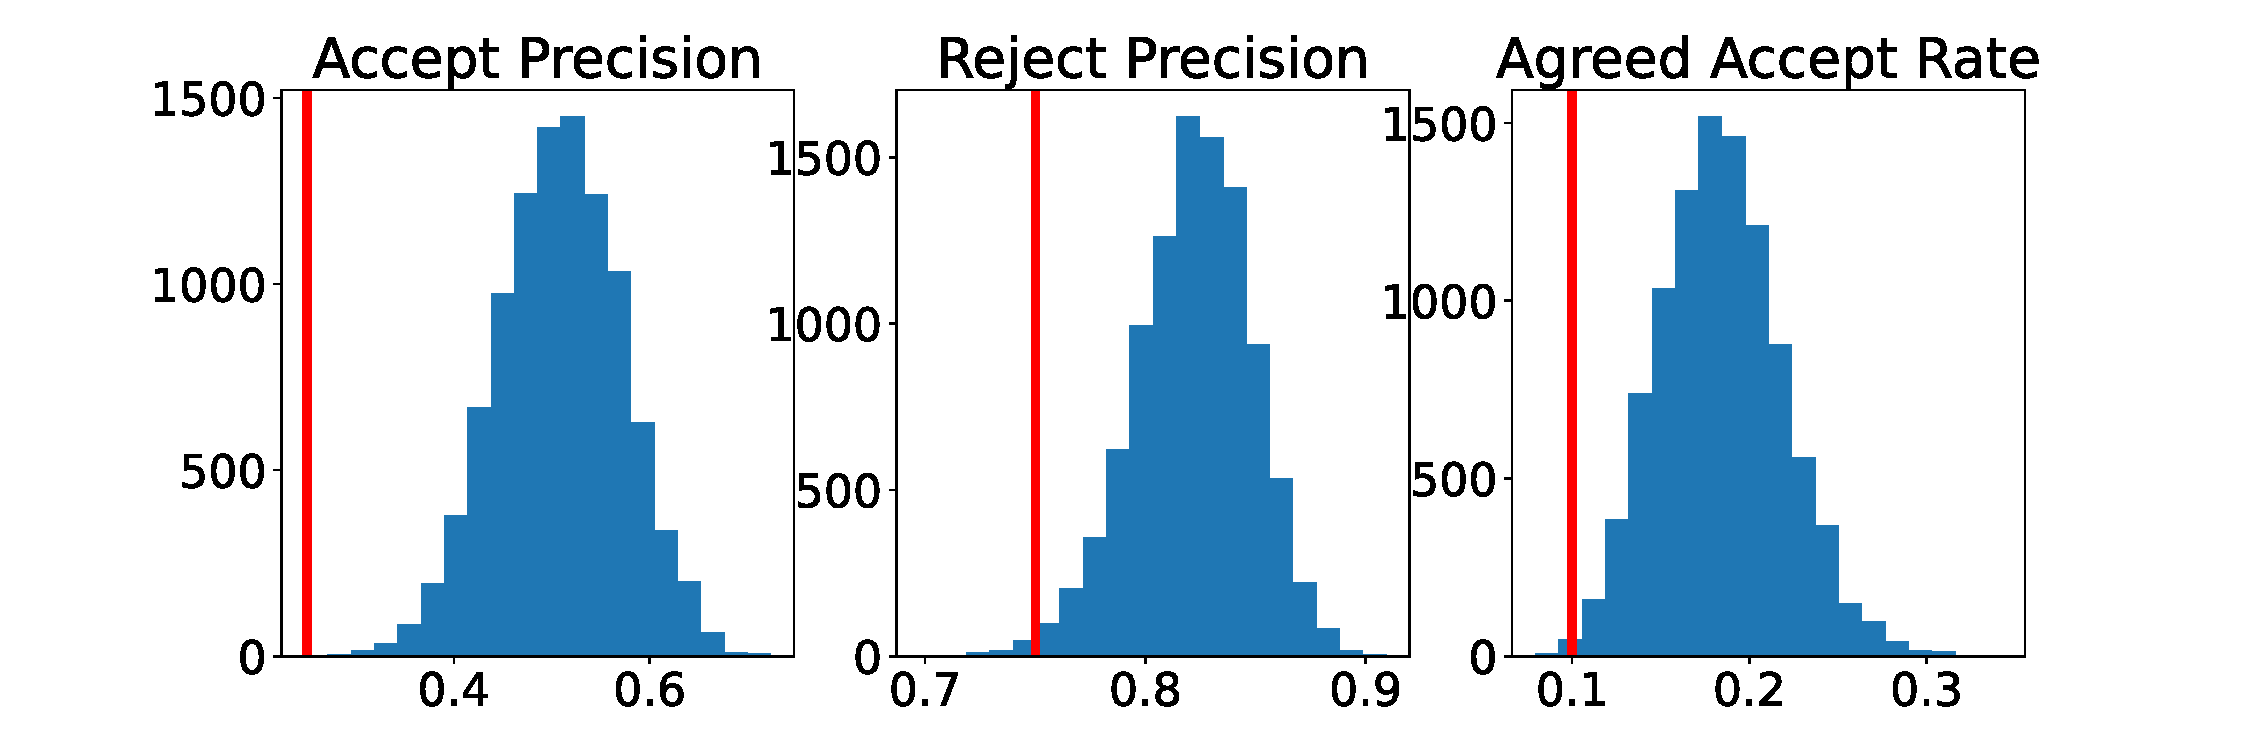
\includegraphics[width=0.90\textwidth]{diagrams/neurips/random-committee-outcomes-vs-true.pdf}


\caption{Different statistics for the random committee outcomes versus the observed committee outcomes. The red lines indicate results from the NeurIPS experiment, the blue histograms are of Monte Carlo samples from the random committee.}
\label{random-committee-outcomes}
\end{figure}

From the histograms, it's clear that the observed statistics we see for the committee in the experiment is at the very low end of the distributions generated by Monte Carlo samples from the random committee.

\subsection{Model Choice and Prior
Values}\label{model-choice-and-prior-values}

In the analysis above we've minimised the modeling choices: we made use
of a Bayesian analysis to capture the uncertainty in counts that can be
arising from statistical sampling error. To this end we chose an
uninformative prior over these probabilities. However, one might argue
that the prior should reflect something more about the underlying
experimental structure: for example, we \emph{know} that if the
committees made their decisions independently it is unlikely that we'd
obtain an inconsistency figure much greater than 37.5\% because that
would require committees to explicitly collude to make inconsistent
decisions: the random conference is the worst case. Due to the accept
rate, we also expect a larger number of reject decisions than reject.
This also isn't captured in our prior. Such questions move us into the
realms of modeling the process, rather than performing a sensitivity
analysis. However, if we wish to model the decision process as a whole,
we have a lot more information available, and we should make use of it.
The analysis above is intended to exploit our randomised experiment to
explore how inconsistent we expect two committees to be. It focuses on
that single question; it doesn't attempt to give answers on what the
reasons for that inconsistency are and how it may be reduced. The
additional maths was needed only to give a sense of the uncertainty in
the figures. That uncertainty arises due to the limited number of papers
in the experiment. The simulation in Section~\ref{sec:simulation-of-subjective-scoring} gives an alternative analysis based on the subjective component of the reviewer quality score.

\section{Effect of Late Reviews}
\label{app:effect-of-late-reviews}

Conference reviews do not all come in at the requested time, the cumulative number of reviews that the conference over time is given in Figure \ref{review-count}.

\begin{figure}[htb]
\centering
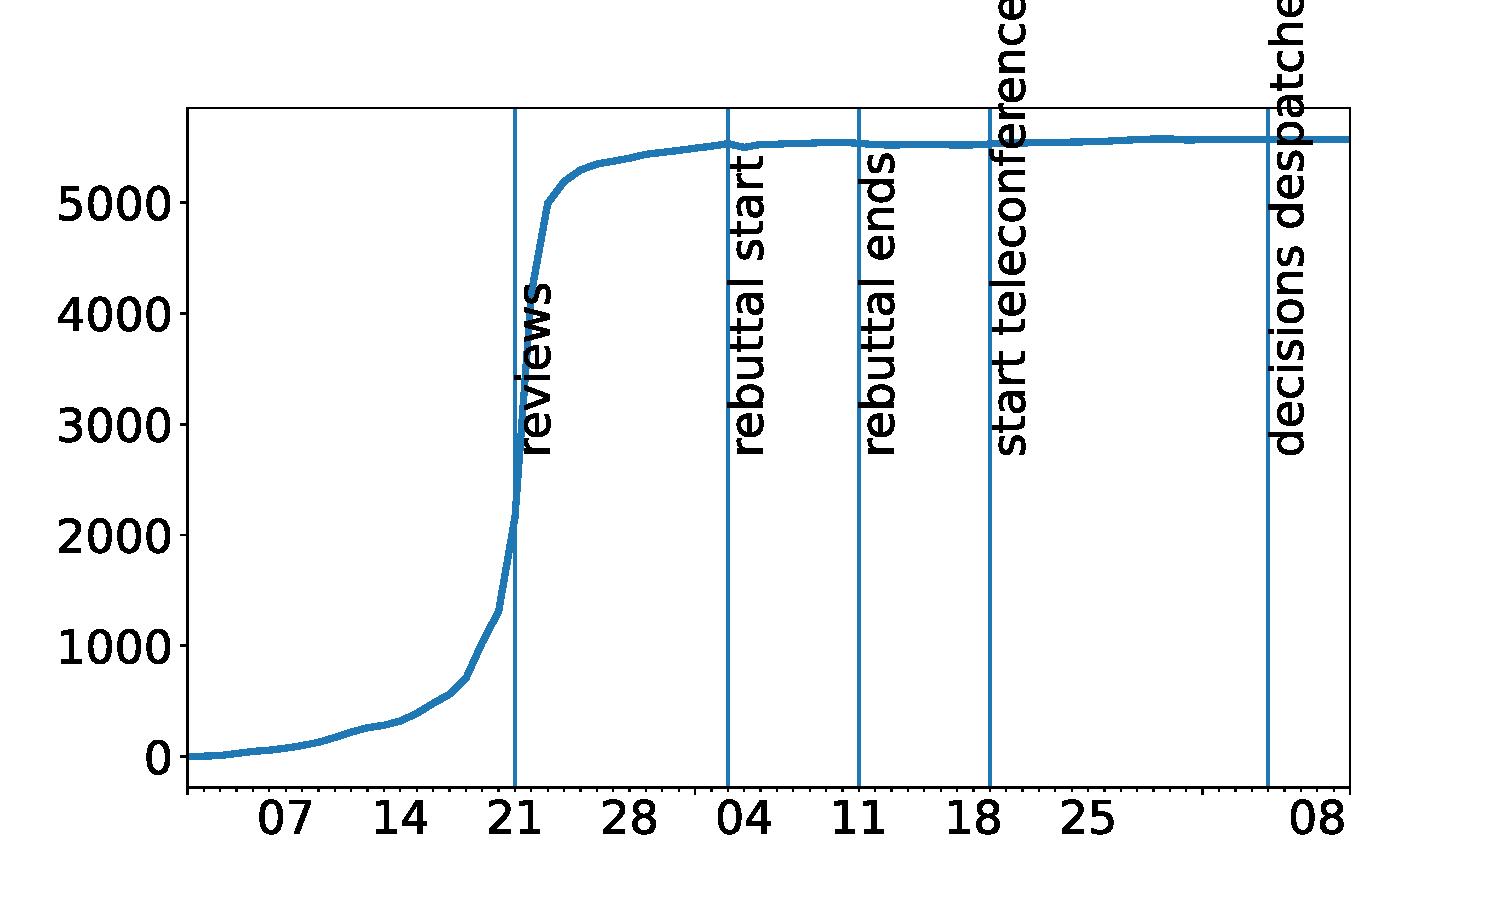
\includegraphics[width=0.70\textwidth]{diagrams/neurips/review-count.pdf}
\caption{Cumulative count of number of received reviews across July and August. Review submission deadline was 21st July.}
\label{review-count}
\end{figure}

The Program Committee worked hard to ensure that all  papers had three reviews
before the start of the rebuttal. In this section we explore differences between late submitted reviews and those submitted on time. Code for recreating this analysis is available in this Jupyter notebook: \url{https://github.com/lawrennd/neurips2014/blob/master/notebooks/NIPS%202014%20Late%20Review%20Observations.ipynb}.  In Figure \ref{number-of-reviews-over-time}  we show the  overall statistics of what the count of reviewers per
paper were, we plot mean, maximum, median, and minimum over time. 

\begin{figure}[htb]
\centering
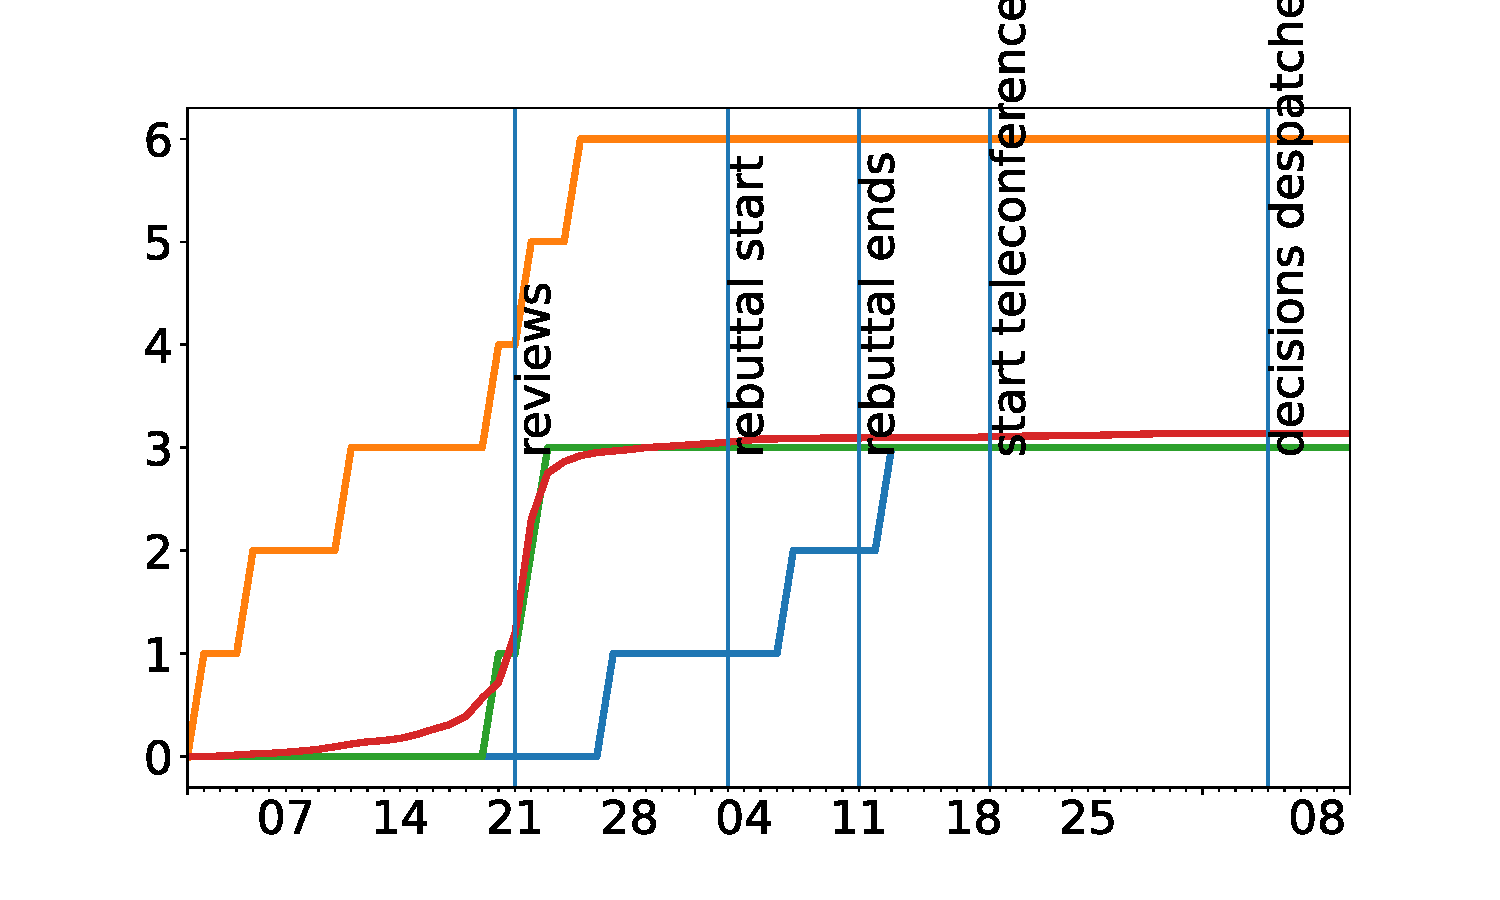
\includegraphics[width=0.70\textwidth]{diagrams/neurips/number-of-reviews-over-time.pdf}

\caption{Plot representing number of reviewers per paper over time showing maximum number of reviewers per paper, minimum, median, and mean. }
\label{number-of-reviews-over-time}
\end{figure}

In Figure~\ref{paper-short-reviews} we show the number of
papers that had less than three reviews across the review period.

\begin{figure}[htb]
\centering
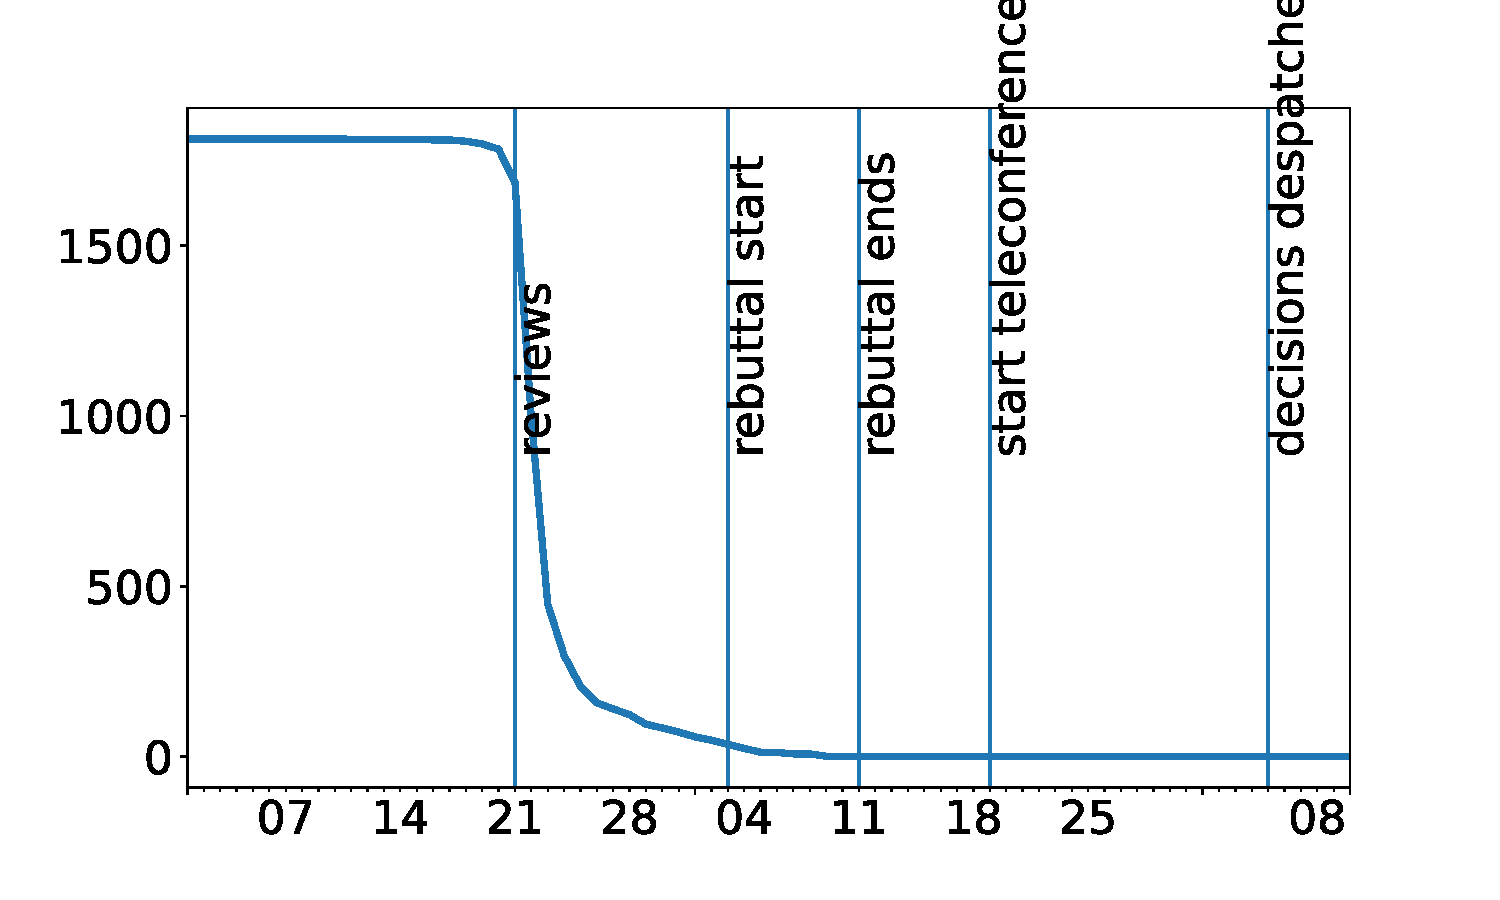
\includegraphics[width=0.70\textwidth]{diagrams/neurips/paper-short-reviews.pdf}

\caption{Number of papers with less than three reviewers as a function of time.}
\label{paper-short-reviews}
\end{figure}

However, while observing the late reviewer scores coming in, the correlation between the two committees reduced (see Figure~\ref{correlation-duplicate-reviews}). Correlation starts high, but it drops as reviewers were chased to submit, then it recovers during the reviewer discussion period. This trend triggered a question: are late reviewers damaging the reviewing process?

\begin{figure}[htb]
\centering
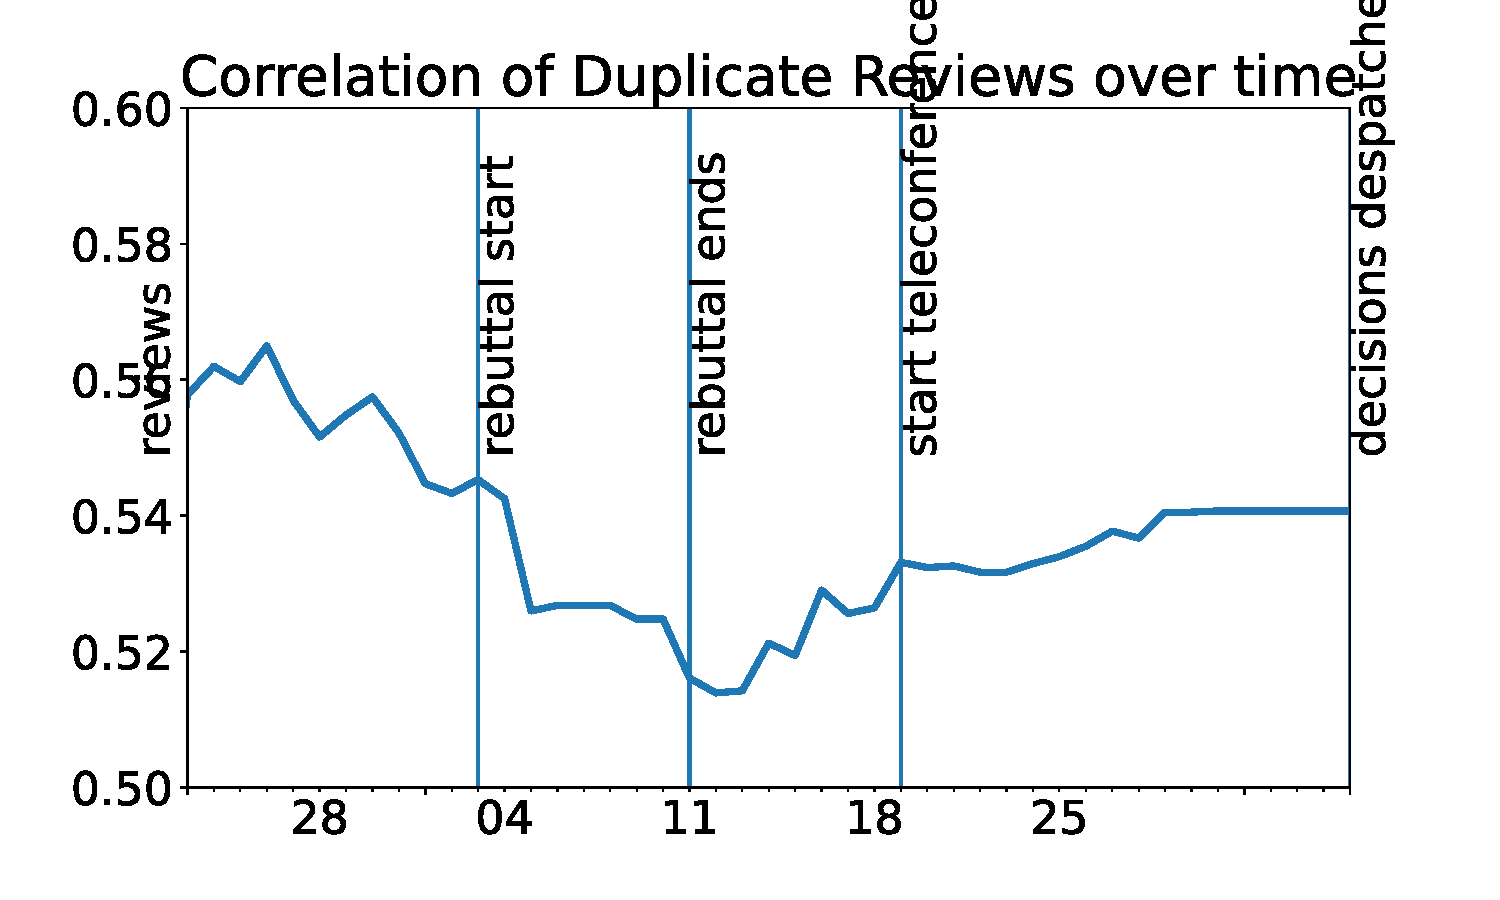
\includegraphics[width=0.70\textwidth]{diagrams/neurips/correlation-duplicate-reviews.pdf}


\caption{Average correlation of duplicate papers over time.}
\label{correlation-duplicate-reviews}
\end{figure}

These changes in correlation were point estimates based on a relatively low number of papers. To get a sense of the uncertainty overtime, we computed bootstrap estimates of the correlation over time. These estimates are shown in Figure~ \ref{correlation-duplicate-reviews-bootstrap}.

\begin{figure}[htb]
\centering
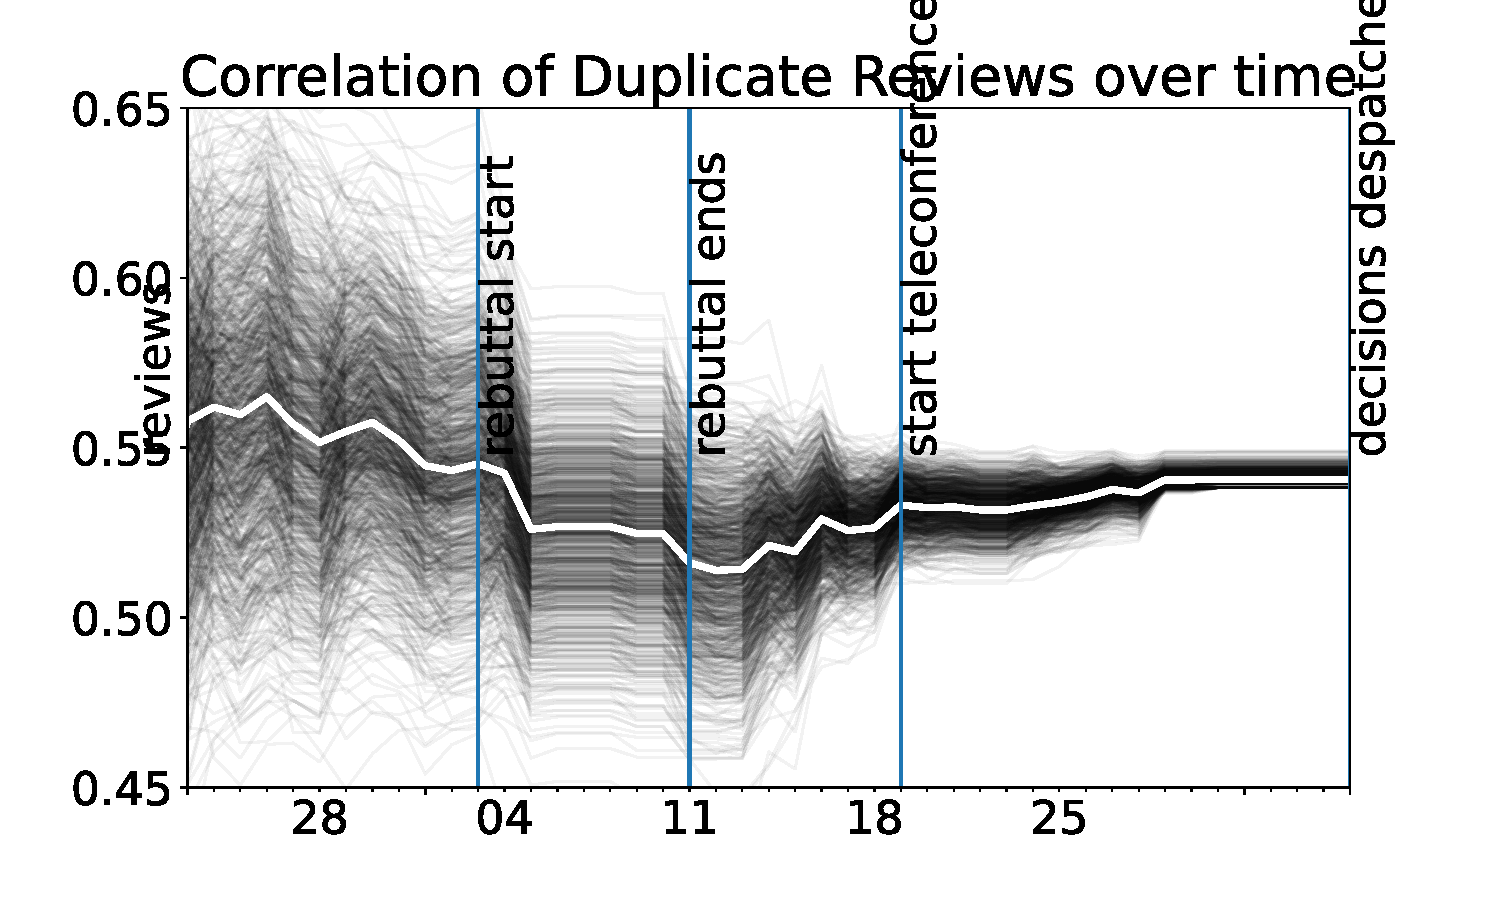
\includegraphics[width=0.70\textwidth]{diagrams/neurips/correlation-duplicate-reviews-bootstrap.pdf}


\caption{Average correlation of duplicate papers over time. To give an estimate of the uncertainty the correlation is computed with bootstrap samples. Here to allow comparison between the trend lines similar, the bootstrap samples are set so they converge on the same point on the right of the graph.}
\label{correlation-duplicate-reviews-bootstrap}
\end{figure}

The bootstrap estimates show how much uncertainty there is in these correlation estimates, and caution us about how much credit to place against any interpretation of these correlations over time, but with curiosity already piqued by the original plot, we decided to compare the quality of reviews between those that were on-time and those that were late.

\subsection{Review Confidence}\label{review-confidence}

First, we consider whether the confidence of reviewes varied over time. We considered a moving four day window across the review submission period and in Figure~\ref{review-confidence-time} we show the mean review confidence over time, alongside 95\% confident intervals computed from the standard errors for the mean estimate. 

\begin{figure}[htb]
\centering
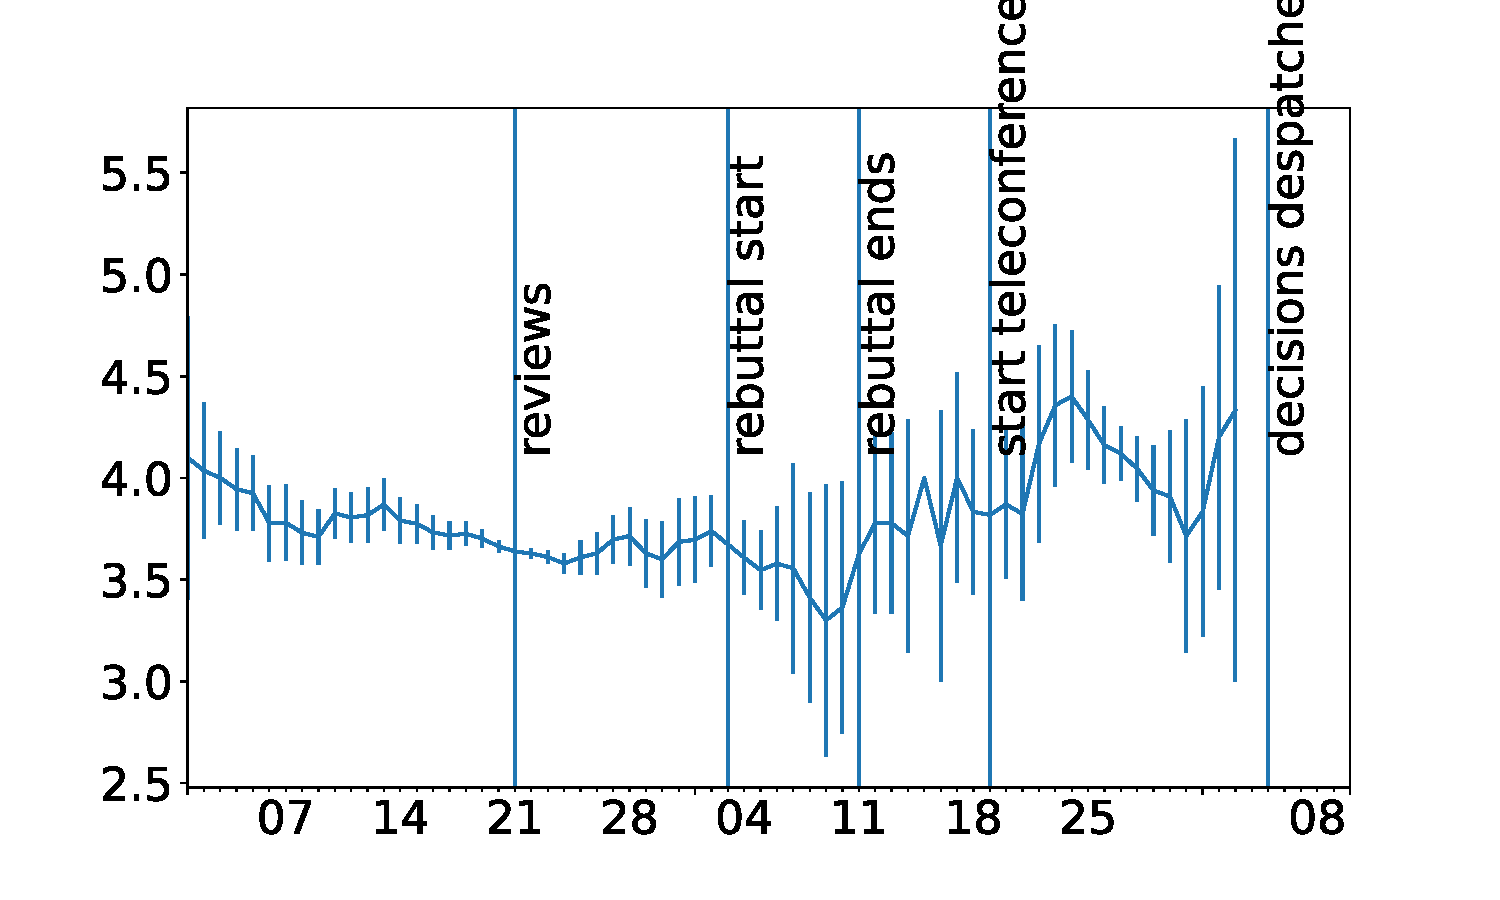
\includegraphics[width=0.70\textwidth]{diagrams/neurips/review-confidence-time.pdf}


\caption{Average confidence of reviews as computed across a four-day moving window, plot includes standard error the mean estimate.}
\label{review-confidence-time}
\end{figure}

Again, a definitive trend is difficult to pick out, but it's plausible that there's a reduction in confidence as we pass the review deadline on 21st July, so the next step was to explore whether that's a statistically significant reduction.

We looked at the average confidence for
reviews that arrived before 21st July (the reviewing deadline) and
reviews that arrived after the 21st July (i.e.~those that were chased or
were allocated late) but before the rebuttal period started (4th
August). In Figure~\ref{review-confidence-early-late} we show the average estimate for these two groups along with error bars from standard error.

\begin{figure}[htb]
\centering
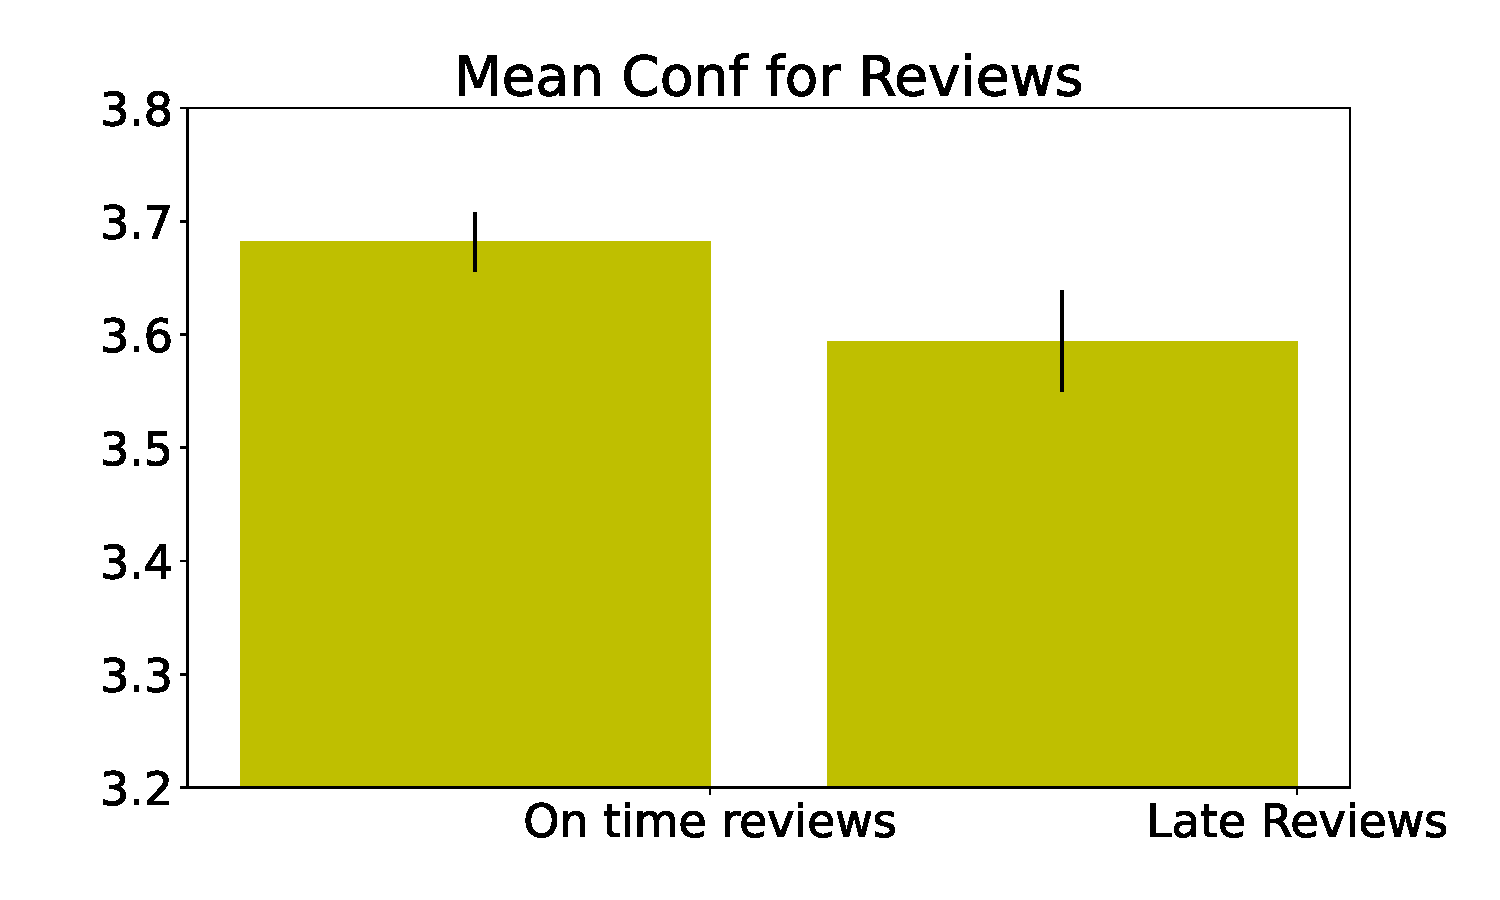
\includegraphics[width=0.50\textwidth]{diagrams/neurips/review-confidence-early-late.pdf}

\caption{Average confidence for reviews that arrived
before 21st July (the reviewing deadline) and reviews that arrived
after. Histogram shows mean values and confidence intervals. A
\(t\)-test shows the difference to be significant with a \(p\)-value of
0.048\%, although the magnitude of the difference is small (about
0.1).} \label{review-confidence-early-late}
\end{figure}

Viewing the plot suggests that there's a small but significant difference between
the average confidence of the submitted reviews before and after the
deadline, the statistical significance is confirmed with a \(t\)-test
with a \(p\)-value at 0.048\%. The magnitude of the difference is small
(about 0.1) but may indicate a tendency for later reviewers to be a
little more rushed.

\subsection{Quality and Impact Scores}\label{quality-score}

Following this analysis around confidence, we performed the same analysis for both the quality scores and the impact scores. The results are shown in Figures
\ref{review-quality-time} and \ref{review-quality-early-late}.

\begin{figure}[htb]
\centering
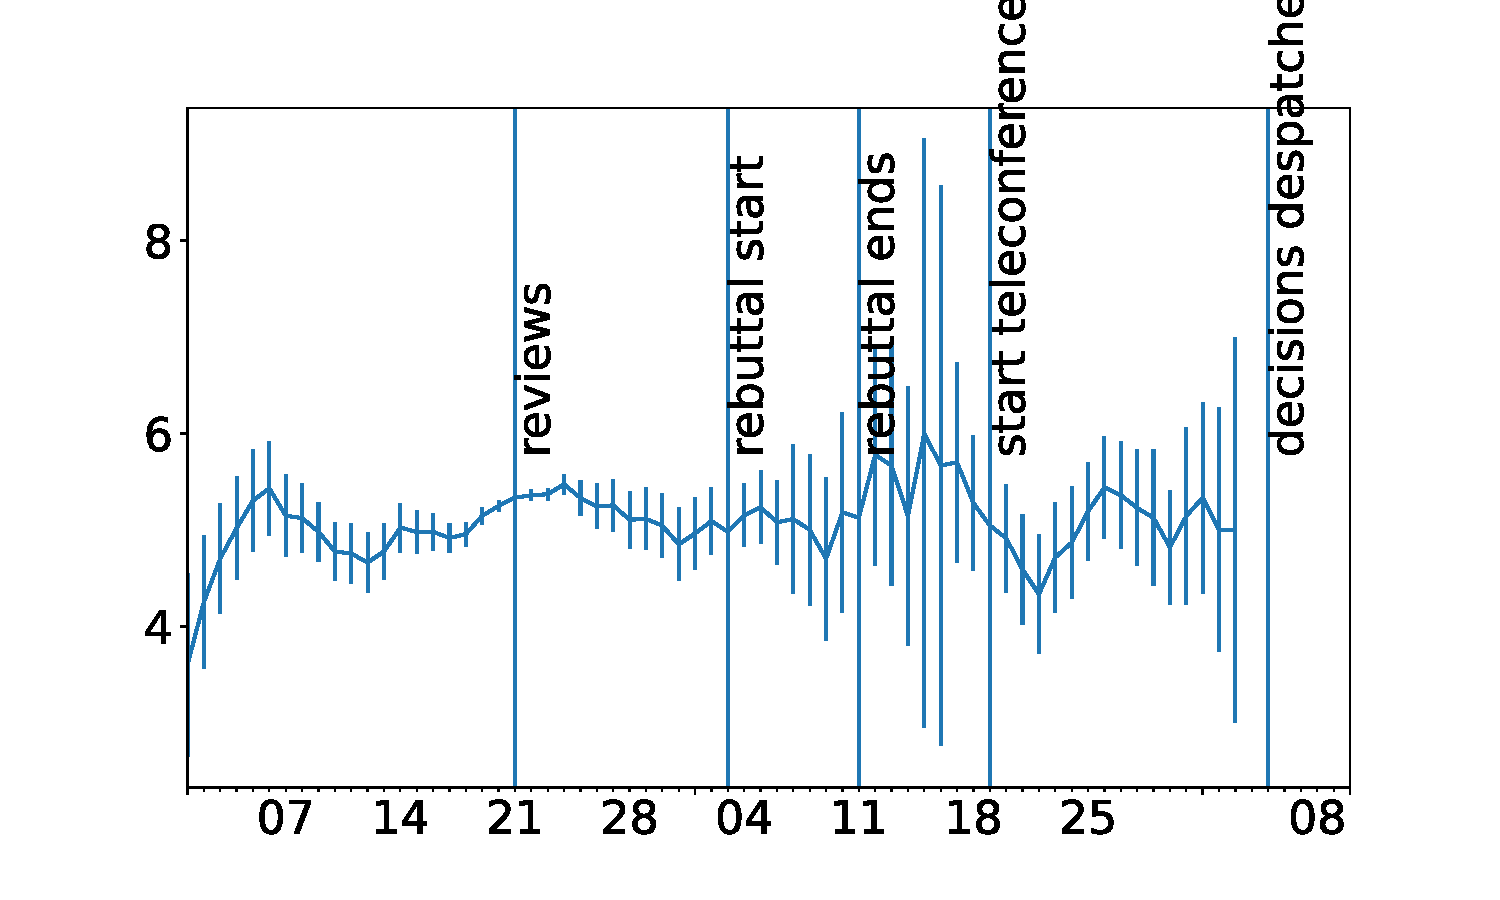
\includegraphics[width=0.70\textwidth]{diagrams/neurips/review-quality-time.pdf}

\caption{Plot of average review quality score as a function of time using a four day moving window. Standard error is also shown in the plot.}
\label{review-quality-time}
\end{figure}

\begin{figure}[htb]
\centering
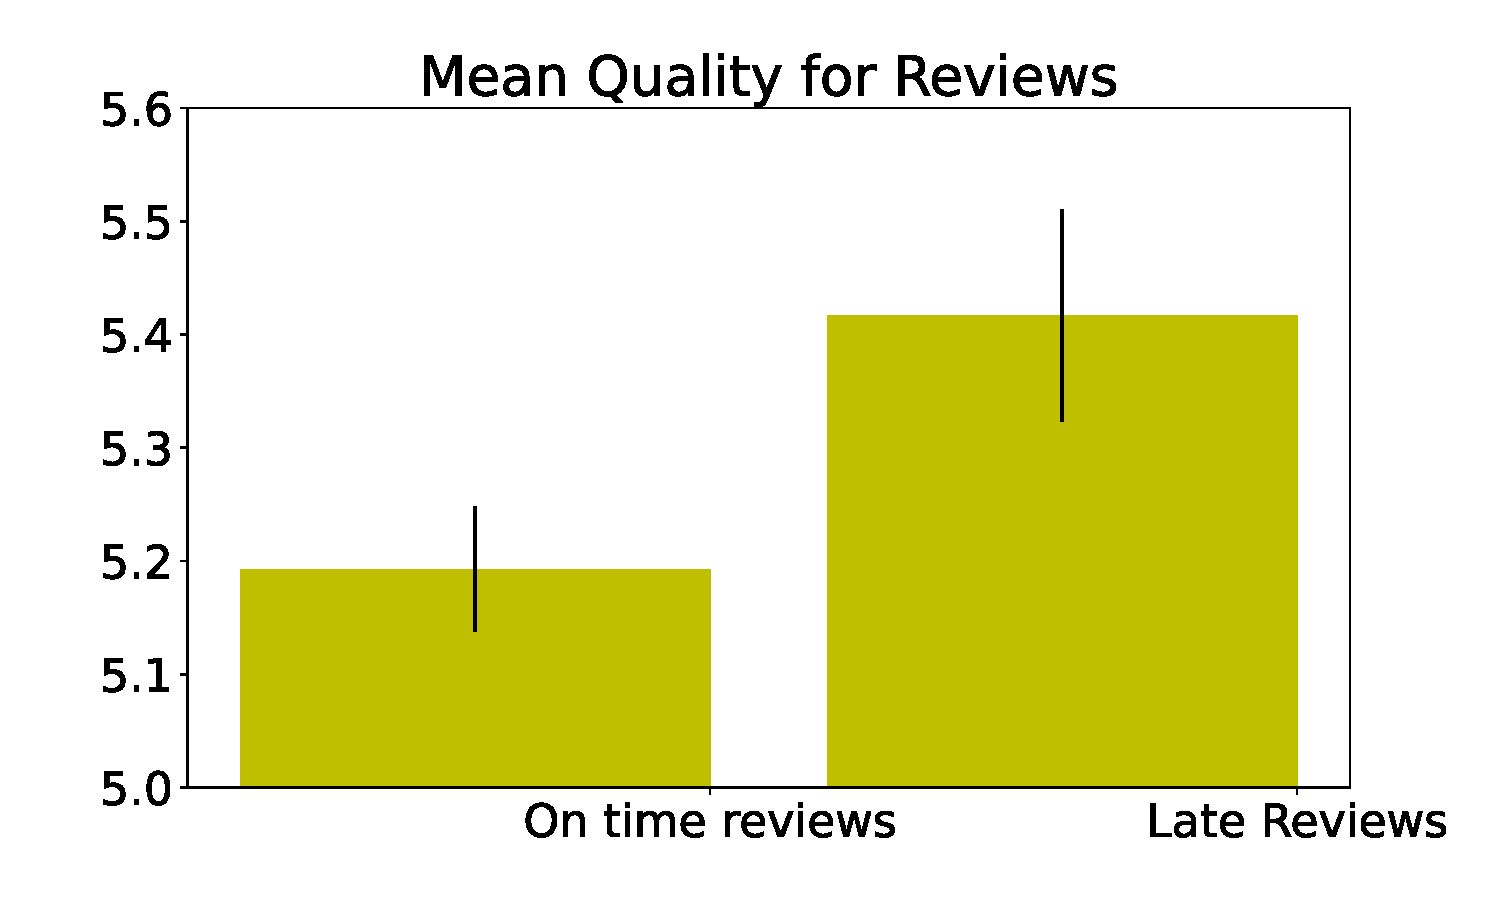
\includegraphics[width=0.50\textwidth]{diagrams/neurips/review-quality-early-late.pdf}

\caption{Bar plot of average quality scores for on-time
reviews and late reviews, standard errors shown. Under a \(t\)-test the
difference in values is statistically significant with a \(p\)-value of
0.007\%.} \label{review-quality-early-late}
\end{figure}

There is another statistically significant difference between perceived
quality scores after the reviewing deadline than before. On average
reviewers tend to be more generous in their quality perceptions when the
review is late. The \(p\)-value is computed as 0.007\%. We can also
check if there is a similar on the impact score (see Section \ref{paper-scoring-and-reviewer-instructions} for more details on the scores). The impact score was
introduced by Ghahramani and Welling in 2013 to get reviewers not just to think
about the technical side of the paper, but whether it is driving the
field forward. The score is binary, with 1 being for a paper that is
unlikely to have high impact and 2 being for a paper that is likely to
have a high impact.

\begin{figure}[htb]
\centering
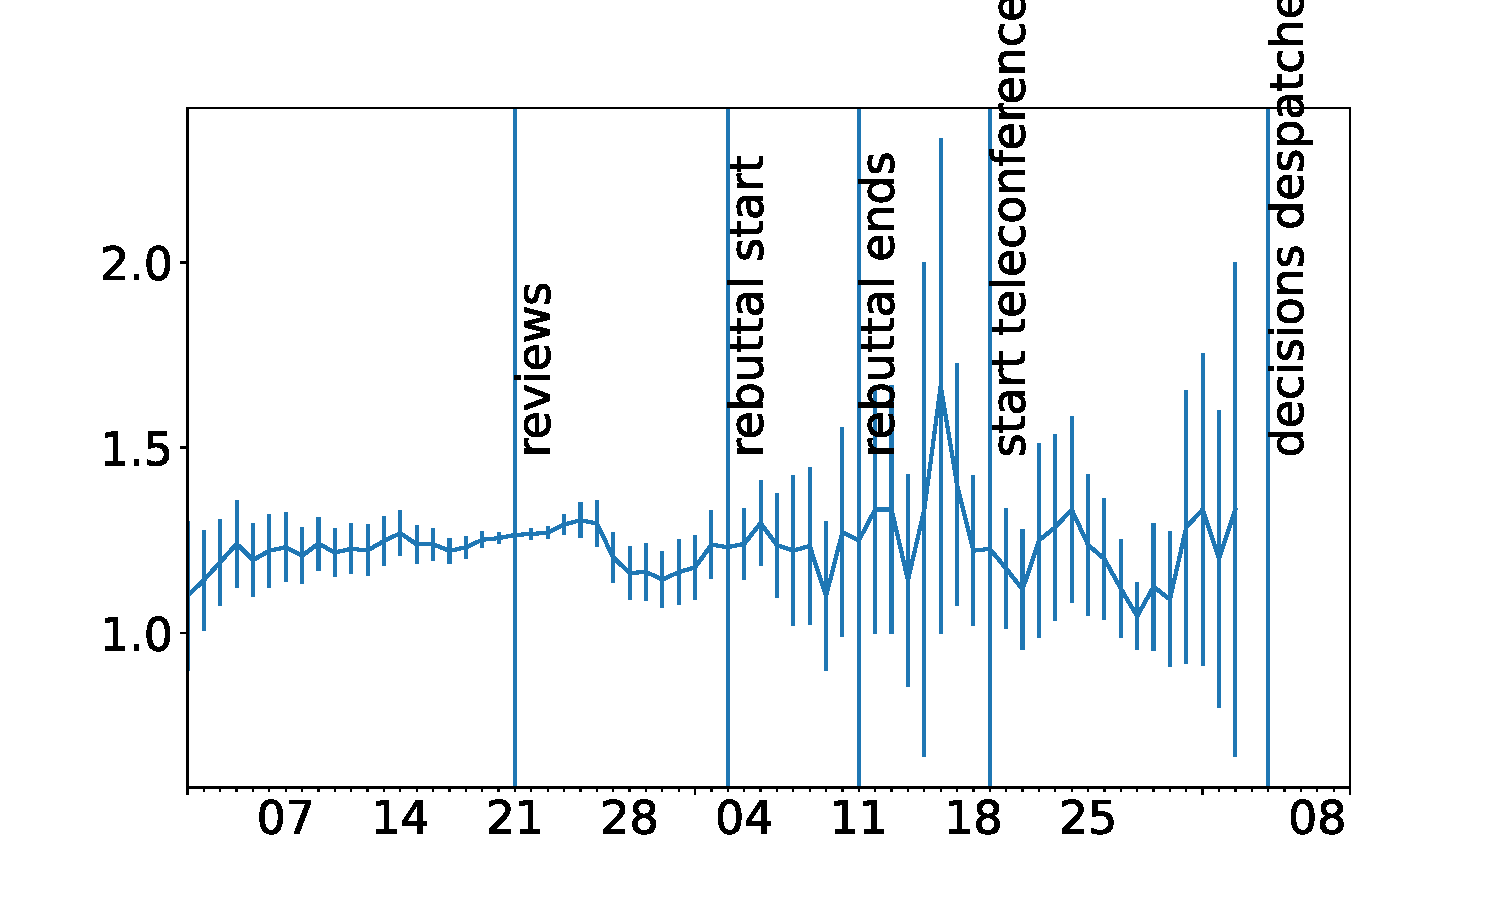
\includegraphics[width=0.70\textwidth]{diagrams/neurips/review-impact-time.pdf}

\caption{Average impact score for papers over time, again using a moving average with a window of four days and with standard error of the mean computation shown.}
\label{review-impact-time}
\end{figure}

\begin{figure}[htb]
\centering
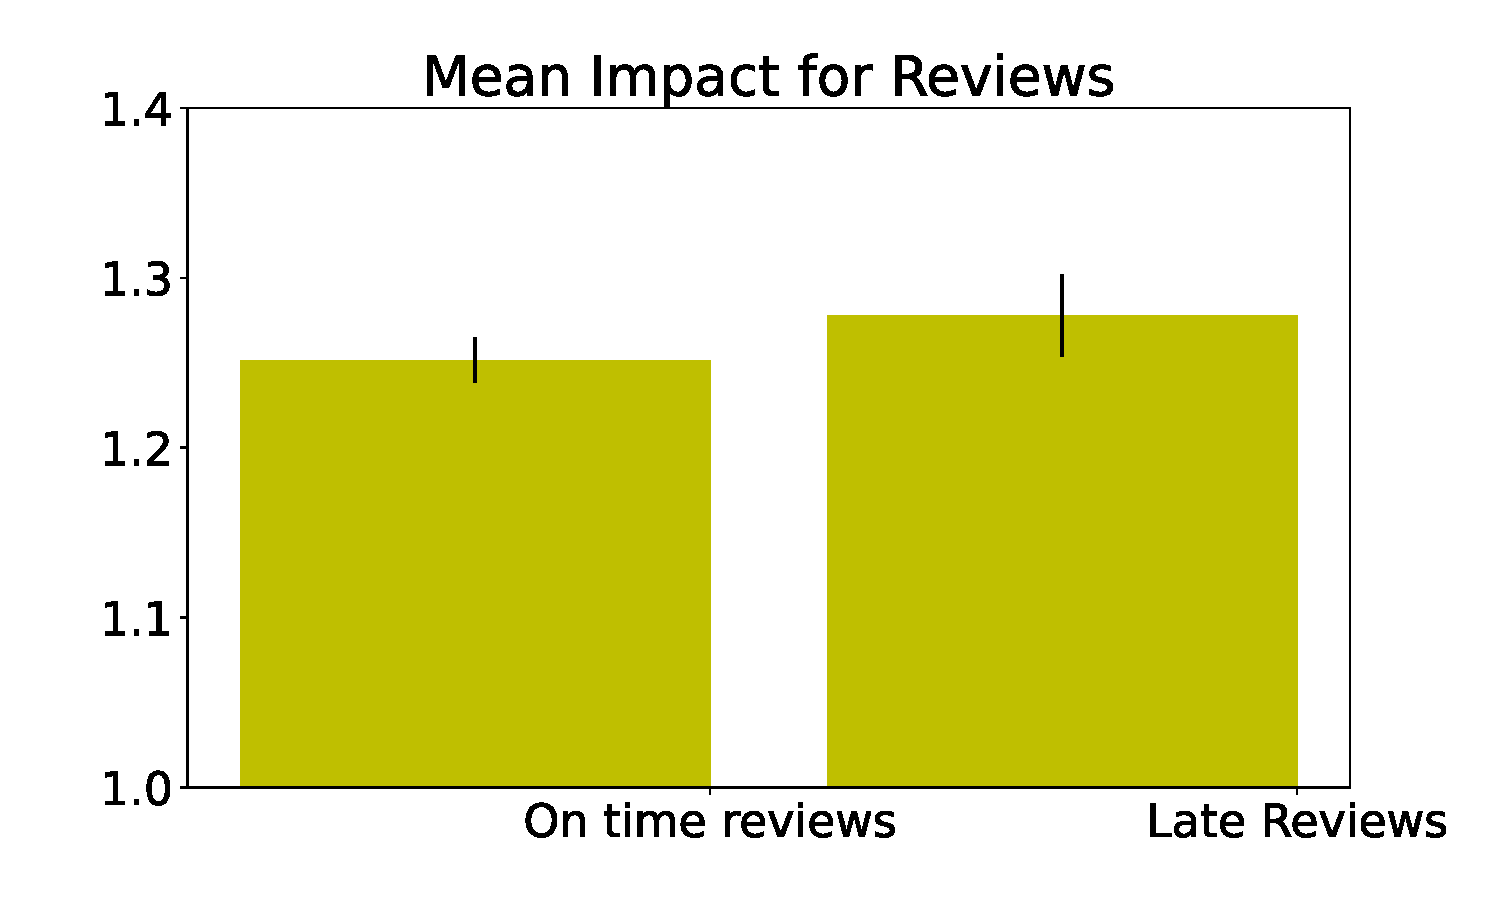
\includegraphics[width=0.50\textwidth]{diagrams/neurips/review-impact-early-late.pdf}

\caption{Bar plot showing the average impact score of
reviews submitted before the deadline and after the deadline. The
difference in means did not prove to be statistically significant under
a \(t\)-test (\(p\)-value 5.9\%).} \label{review-impact-early-late}
\end{figure}

We find the difference is not quite statistically significant for the
impact score (\(p\)-value of 5.9\%), but if anything, there is a trend
to have slightly higher impacts for later reviews (see Figures
\ref{review-impact-time} and \ref{review-impact-early-late}).

\subsection{Review Length}\label{review-length}

A final potential indicator of the review quality is the length of the
reviews, we can check if there is a difference between the combined
length of the review summary and the main body comments for late and
early reviews (see Figures \ref{review-length-time} and
\ref{review-length-early-late}).

\begin{figure}[htb]
\centering
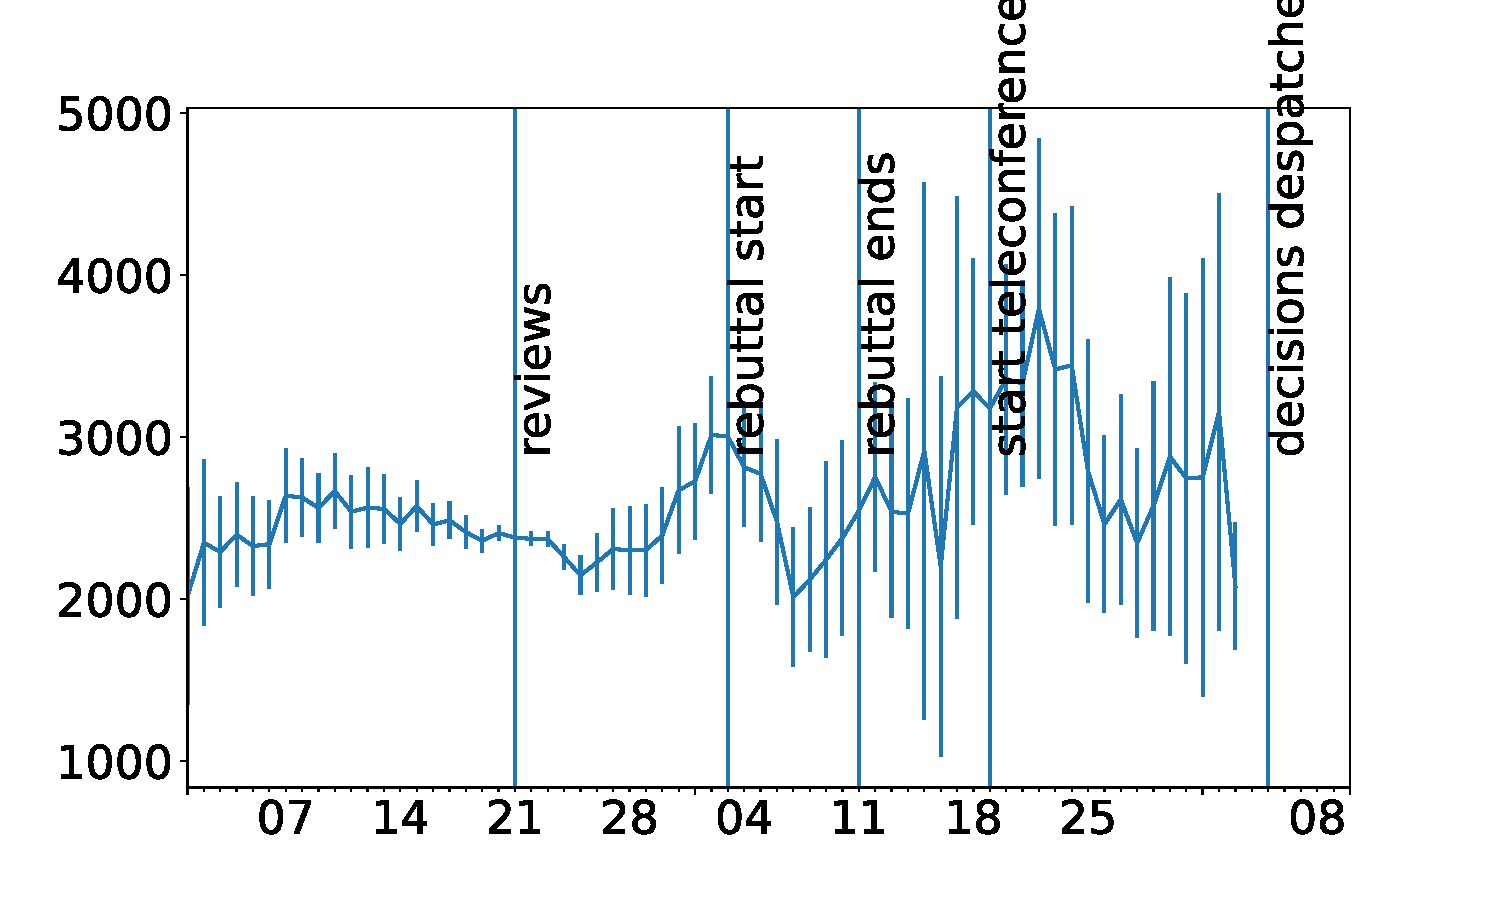
\includegraphics[width=0.70\textwidth]{diagrams/neurips/review-length-time.pdf}


\caption{Average length of reviews submitted plotted as a function of time with standard error of the mean computation included.}
\label{review-length-time}
\end{figure}

\begin{figure}[htb]
\centering
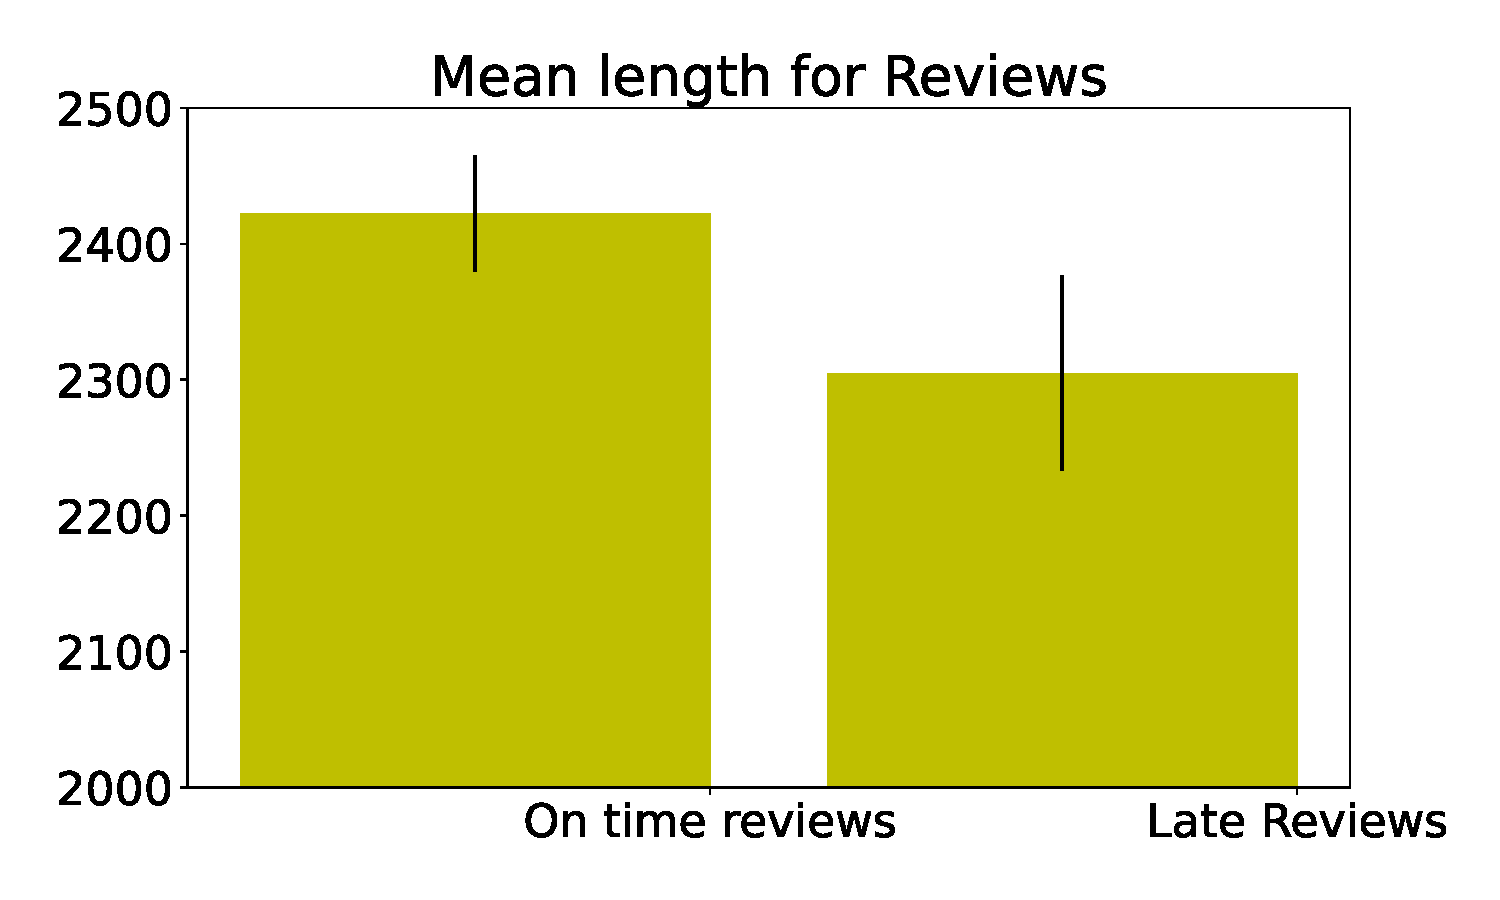
\includegraphics[width=0.50\textwidth]{diagrams/neurips/review-length-early-late.pdf}

\caption{Bar plot of the average length of reviews
submitted before and after the deadline with standard errors included.
The difference of around 100 words is statistically significant under a
\(t\)-test (\(p\)-value 0.55\%).} \label{review-length-early-late}
\end{figure}

Once again we find a small but statistically significant difference,
here, as we might expect late reviews are shorter than those submitted
on time, by about 100 words in a 2,400 word review.


\subsection{Late Reviewers Summary}\label{late-reviewers-summary}

In summary we find that late reviews are on average less confident and
shorter, but rate papers as higher quality and perhaps as higher impact.
Each of the effects is small (around 5\%) but overall a picture emerges
of a different category of review arriving from those that delay their
assessment.

\section{Correlation of Quality Scores and
Citation}\label{correlation-of-quality-scores-and-citation}

To revisit the NeurIPS experiment, we traced the fate of accepted papers and all the rejected papers that we could find through searching on Semantic Scholar. This allowed us to associate each paper with a citation count. In this section we explore correlation between those citation counts and the scores that reviewers gave the papers back in 2014.

Code that traces the fate of rejected papers (in terms of their final publication venue) can be found in this Jupyter notebook: \url{https://github.com/lawrennd/neurips2014/blob/master/notebooks/where-do-rejected-papers-go.ipynb} and code that computes the citation scores and compares them to quality scores can be found in this Jupyter notebook: \url{https://github.com/lawrennd/neurips2014/blob/master/notebooks/Measuring%20Impact%20of%20Papers%20Using%20Semantic%20Scholar.ipynb}.

First of all, we plot the correlation between average quality score and the citation count for all papers where we could trace their fate (accepted and rejected). This is shown in  Figure~\ref{figure-citations-vs-average-calibrated-quality-all}. Rejected papers are given as crosses,
accepted papers are given as dots. We include all papers, whether
published in a venue or just available through ArXiv or other preprint
servers. We show the published/non-published quality scores and
\(\log_{10}(1+\text{citations})\) for all papers in the plot below. In
the plot we are showing each point corrupted by some Laplacian noise and
also removing axes. The idea is to give a sense of the distribution
rather than reveal the score of a particular paper.

\begin{figure}[htb]
\centering
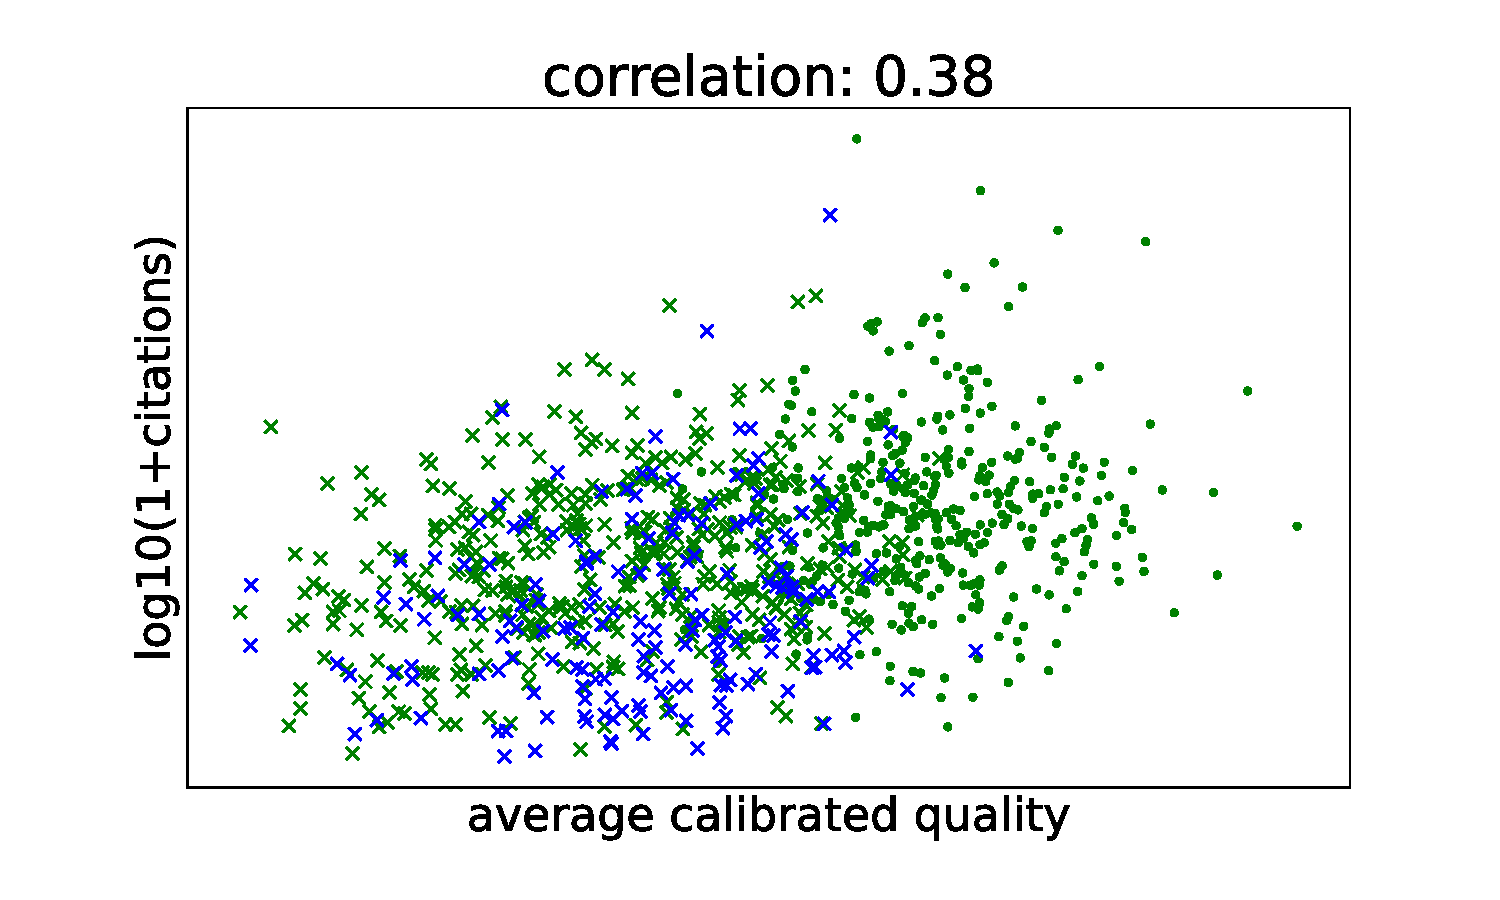
\includegraphics[width=0.70\textwidth]{diagrams/neurips/citations-vs-average-calibrated-quality-all.pdf}


\caption{Scatter plot of $\log_{10}(1+\text{citations})$ against the average calibrated quality score for all papers. To prevent reidentification of individual papers quality scores and citation count, each point is corrupted by differentially private noise in the plot (correlation is computed before adding differentially private noise). Rejected papers are given as crosses, accepted papers are shown as dots. Papers that found a venue are shown in green. Any paper that is only available through pre-print servers or as an unpublished PDF is shown in blue.}
\label{figure-citations-vs-average-calibrated-quality-all}
\end{figure}

The correlation between the reviewer scores and the citation impact score looks strong, but there is a counfounder here because we've bundled together papers that were accepted and those that were rejected from the conference. Papers accepted by the conference will have been published earlier and presentation at the conference is likely to have given a  lift to the papers' numbers of citations. So, we analyze these two groups separately.

Looking at the accepted papers only shows a very different picture. As outlined in the main text, 
there is no statistically significant correlation between accepted papers' quality scores
and the number of citations they receive (see Figure \ref{figure-citations-vs-average-calibrated-quality-accept}). 

Conversely, looking at rejected papers only, we do see a correlation (Figure~\ref{figure-citations-vs-average-calibrated-quality-reject}),
with higher scoring papers achieving more citations on average. This,
combined with the lower average number of citations in the rejected
paper group, alongside their lower average scores, explains the
correlation we observed when analyzing the two groups of papers together.

Welling and Ghahramani introduced an ``impact'' score in NeurIPS 2013,
we might expect the impact score to show correlation. And indeed,
despite the lower range of the score (a reviewer can score either 1 or
2) we do see \emph{some} correlation, although it is relatively weak (Figure \ref{figure-citations-vs-average-impact-accept}).


Finally, we also looked at correlation between the \emph{confidence}
score and the citation count. Here correlation is somewhat stronger (0.25) and is statistically significant (see Figure~\ref{figure-citations-vs-average-confidence-accept}). Why should
confidence be an indicator of higher citations? A plausible explanation
is that there is confounder driving both variables. For example, it
might be that papers which are easier to understand (due to elegance of
the idea, or quality of exposition) inspire greater reviewer confidence
and increase the number of citations.


%%%%%%%%%%  End Body  %%%%%%%%%%
